\documentclass{pracamgr}
\usepackage{polski}
\usepackage[utf8]{inputenc}
\usepackage{amssymb}
\usepackage{amsmath}
\usepackage{amsthm}
\usepackage[pdftex]{graphicx}
\usepackage{multicol}
\usepackage{hyperref}

\author{Wiktor Zuba}

\nralbumu{320501}

\title{Efektywne algorytmy generacji obiektów kombinatorycznych???}

\tytulang{Effective algorithms of combinatorial objects generation???}

\kierunek{Informatyka}

\opiekun{prof. Wojciech Rytter\\
Instytut Informatyki}

\date{??? 2017}

\dziedzina{ 
 ???
}


\klasyfikacja{
???
}

\keywords{???}

\newtheorem{defi}{Definicja}[section] %TODO może wprowadzić nową rzecz - oznaczenie np. dla [n], czy u\Delta v
\newtheorem{theorem}{Twierdzenie}
\newtheorem{conjecture}{Przypuszczenie}
\newtheorem{lemma}[theorem]{Lemat}
\newtheorem{remark}[theorem]{Uwaga}
\newtheorem{fact}[theorem]{Fakt}
\newtheorem{corollary}[theorem]{Wniosek}


\begin{document}
\maketitle

\begin{abstract}
???
\end{abstract}

%TODO część dwudzielna - jak coś należy do jednej części - wypada to jakoś inaczej nazywać
%monopartite, bipartial,      mowa też o bipartycji U,V
%TODO hamiltonian laceable? - jak przetłumaczyć

\tableofcontents%TODO podać, że overline coś to wektor, równy x_1,x_2,...,x_l plus może , overline0 to wektor z samych zer





 \chapter*{Wprowadzenie}
 \addcontentsline{toc}{chapter}{Wprowadzenie}
  
 \chapter{Własności hiperkostki}
  \section{Podstawowe definicje}
   \begin{defi}\label{[n]}
    Dla $n\in\mathbb{N}$\quad $[n]=\{0,...,n-1\}$ (zbiór pierwszych $n$ liczb naturalnych).
   \end{defi}
   \subsection{Hiperkostka}
    \begin{defi}\label{hiperkostka}
     \emph{Hiperkostką wymiaru $n$ ($Q_n$)} nazwiemy graf, w którym każdy wierzchołek odpowiada ciągowi binarnemu długości $n$,
     zaś krawędzią połączone są te wierzchołki, których ciągi binarne różnią się na dokładnie jednej pozycji.\newline
     $V(Q_n)=\{(v_0,...,v_{n-1}):v_i\in\{0,1\}\}, E(Q_n)=\{(u,v):\sum_{i}|u_i-v_i|=1\}$
    \end{defi}
    \begin{center}
     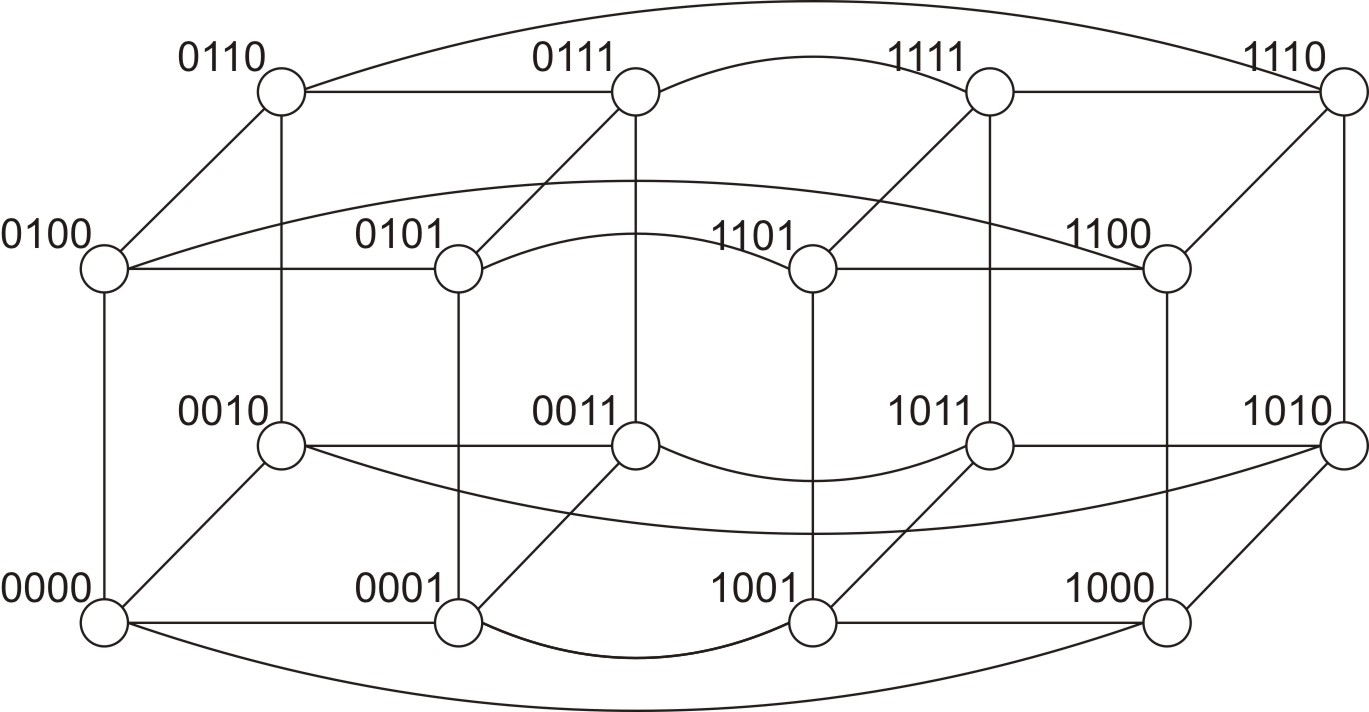
\includegraphics[scale=0.6]{img/Q_4.jpg}
    \end{center}
    W przypadku pełnej hiperkostki
    bardzo łatwo jest określić długość najkrótszej ścieżki pomiedzy wierzchołkami --
    jest ona równa ilości pozycji na których różnią się ciągi tych wierzchołków.\newline
    Hiperkostka jest grafem dwudzielnym, w którym jedną składową jest zbiór wierzchołków o ciągach z parzystą liczbą jedynek,
    zaś drugą tych o ich nieparzystej liczbie.\newline
    Co więcej przy badaniu hiperkostek często dzieli się je na $n+1$ warstw, gdzie dla $i\in[n+1]$ $i$-tą warstwę stanowią te wierzchołki,
    których ciągi binarne mają dokładnie $i$ jedynek (warstwa zawiera zatem wierzchołki oddalone o $i$ od wierzchołka zerowego ($\overline{0}$)).
    \begin{defi}\label{delta wierzcholkow}
     Dla dwóch wierzchołków hiperkostki defininiujemy:
     $u\Delta v=\{i:u_i\neq v_i\}$, gdzie $(u_0,...u_{n-1})$ i $(v_0,...,v_{n-1})$ to ciagi binarne wierzchołków $u$ i $v$ odpowienio
     ($|u\Delta v|$ wyznacza odległość wierzchołków w hiperkostce).
    \end{defi}
    \begin{defi}\label{numerowanie klasyczne}
     \emph{Numerowaniem klasycznym (naturalnym)} hiperkostki nazwiemy takie numerowanie $\varphi:V(Q_n)\rightarrow\{1,...,|V(Q_n)|\}$ jej wierzchołków, że
     $\varphi(v)=1+\sum_{i}v_i\cdot2^i$
    \end{defi}
    \begin{center}
     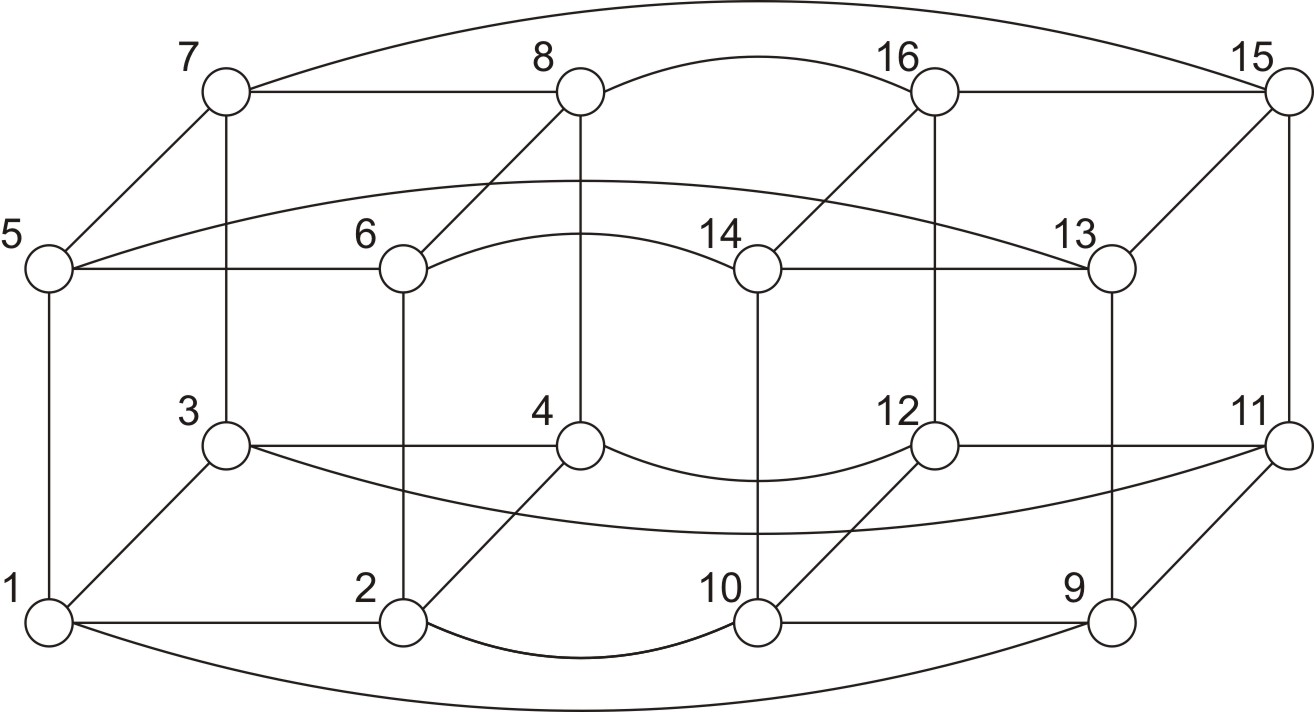
\includegraphics[scale=0.6]{img/Q_4_klasyczne.jpg}
    \end{center}
    \begin{defi}\label{numerowanie warstwowe}%TODO może n choose -1 nie jest tak bardzo standardowe
     \emph{Numerowaniem warstwowym} hiperkostki nazwiemy jej numerowanie w kolejności przeszukiwania grafu wszerz zaczynając od wierzchołka $\overline{0}$
     z wybieraniem sąsiadów w kolejności leksykograficznej.
    \end{defi}
    \begin{center}
    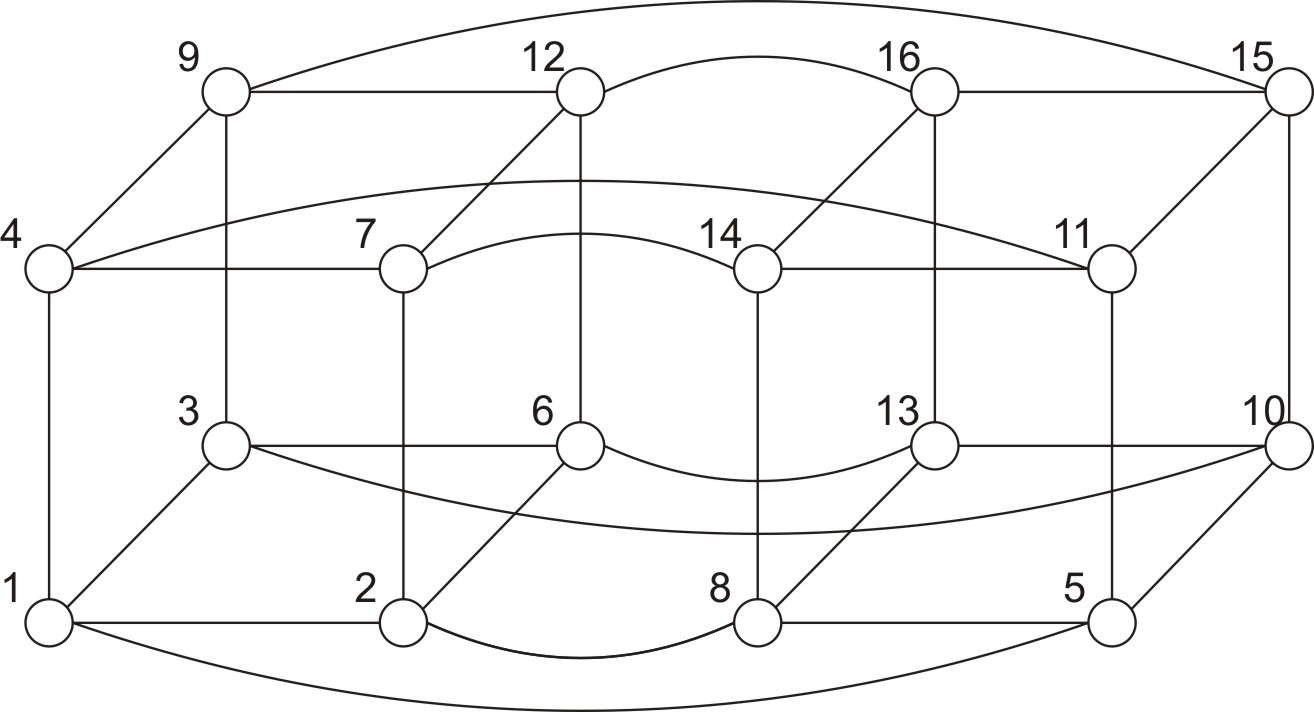
\includegraphics[scale=0.6]{img/Q_4_warstwowe.jpg}
   \end{center}   
    \begin{remark}\label{numerowanie warstwowe 2}
     Jest to takie numerowanie $\varphi:V(Q_n)\rightarrow\{1,...,|V(Q_n)|\}$ jej wierzchołków,
     że wierzchołki z $i$-tej warstwy otrzymują numery od $\sum_{j=0}^{i-1}{n\choose j}+1$ do $\sum_{j=0}^{i}{n\choose j}$.
     W obrębie jednej warstwy numery przyznawane są przeciwnie do kolejności leksykograficznej na odwróconych słowach.
     $\varphi(v)>\varphi(u)\Leftrightarrow (\sum_{i=0}^n v_i>\sum_{i=0}^n u_i)
     \vee((\sum_{i=0}^n v_i=\sum_{i=0}^n u_i)\wedge(\sum_{i=0}^n2^{n-i}v_i<\sum_{i=0}^n2^{n-i}u_i))$
    \end{remark}
    \begin{proof}
     Indukcyjnie po warstwach.\newline
     Dla warstwy $0$ oczywiste.\newline
     Zakładając, że $i$-ta warstwa jest ponumerowana w tym porządku weźmy dwa wierzchołki $u,v$ z warstwy $i+1$:
     $u=(\overline{y_1},1,\overline{x}),v=(\overline{y_2},0,\overline{x})$.\newline
     Jeśli $\overline{y_1}$ zawiera same $0$, to $\overline{y_2}$ zawiera dokładnie jedną $1$, sąsiedzi tych wierzchołków z poprzedniej warstwy
     o namniejszych numerach to odpowiednio $(\overline{0},0,x),(\overline{0},0,x)$,
     tak więc zostaną ponumerowane jako sąsiedzi tego samego wierzchołka, jednak $u$ otrzyma mniejszy numer jako sąsiad mniejszy leksykograficznie.\newline
     Jeśli $\overline{y_1}$ zawiera $1$, to $\overline{y_2}$ też, więc sąsiedzi tych wierzchołków z poprzedniej warstwy
     o namniejszych numerach to odpowiednio $(\overline{y'_1},1,\overline{x}),(\overline{y'_2},0,\overline{x})$, gdzie $\overline{y'_1}$ i $\overline{y'_2}$,
     to odpowiednio $\overline{y_1}$ i $\overline{y_2}$ z pierwszymi $1$ zamienionymi na $0$. Z założenia indukcyjnego sąsiad $u$ ma mniejszy numer niż sąsiad $v$,
     więc $u$ ma mniejszy numer niż $v$.
    \end{proof}
   \subsection{Sąsiedztwo}
    \begin{defi}\label{sasiedztwo wierzcholka}
     Dla grafu $G$ oraz wierzchołka $v\in V(G)$ definiujemy \emph{sąsiedztwo wierzchołka} jako zbiór wierzchołków połączonych z nim krawędzią:
     $N(v)=\{u\in V(G):(u,v)\in E(G)\}$.
    \end{defi}
    \begin{defi}\label{sasiedztwo zbioru wierzcholkow}%TODO może jakieś lepsze przetłumaczenie boundary
     Dla grafu $G$ oraz zbioru wierzchołków $S\subseteq V(G)$ definiujemy \emph{sąsiedztwo zbioru wierzchołków} jako zbiór tych sąsiadów wierzchołków ze zbioru,
     które same do tego zbioru nie należą: $N(S)=(\bigcup_{v\in S}N(v))\backslash S$
    \end{defi}
    \begin{defi}\label{wnetrze zbioru wierzcholkow}
     Dla grafu $G$ oraz zbioru wierzchołków $S\subseteq V(G)$ definiujemy \emph{wnętrze zbioru wierzchołków} jako zbiór tych wierzchołków z $S$,
     których wszyscy sąsiadzi również należą do tego zbioru: $In(S)=\{v\in S:N(v)\subseteq S\}$
    \end{defi}
   \subsection{Podgrafy}
    \begin{defi}\label{podgraf indukowany}
     Dla danego $V\subseteq V(G)$\quad $G[V]=(V,\{uv\in E(G):u,v\in V\})$ oznacza \emph{podgraf indukowany} przez podzbiór wierzchołków $V$.
    \end{defi}
    \begin{defi}\label{roznica grafow}
     Dla danego $V\subseteq V(G)$\quad $G-V=G[V(G)\backslash V]$ oznacza \emph{graf $G$ z usuniętymi wierzchołkami $V$}.
    \end{defi}
    \begin{defi}\label{kwadrat grafu}
     Dla danego grafu $G$\newline $G^2=(V(G),E(G)\cup\{uv:\exists_{w\in V(G)}uw\in E(G)\cap wv\in E(G)\})$
     oznacza \emph{kwadrat grafu}, czyli graf z dodanymi krawędziami między wierzchołkami oddalonymi o co najwyżej 2.
    \end{defi}
   \subsection{Graf z wadami}
    \begin{defi}\label{graf z wadami}
     W grafie $G$ możemy wyróżnić niektóre wierzchołki (czasem również krawędzie) i oznaczyć jako wadliwe.
     Graf z niepustym takim wyróżnionym zbiorem wierzchołków wadliwych $F\subseteq V(G)$ nazywamy \emph{grafem z wadami} (lub \emph{grafem wadliwym})
    \end{defi}%TODO może dodać wspomnienie, że wadliwy też nazywany usuniętym
    Wadliwe wierzchołki (i/lub krawędzie) najczęściej traktowane są jako usunięte z grafu -- mówimy w tym przypadku o grafie $G-F$.
    Wyróżnianie wadliwych wierzchołków w grafie zamiast definiowania nowego grafu jest umotywowane głównie w przypadkach,
    gdy pełny graf łatwo zdefiniować i zapisać w pamięci małej względem jego rozmiaru (np. klika, hiperkostka, graf de Bruijna),
    a zbiór wadliwych wierzchołków jest również mały.
  \section{Podstawy kombinatoryczne}
   %Wzor Stirlinga: $n!=\sqrt{2\pi n}(\frac{n}{e})^n e^{\lambda_n}$\quad $\frac{1}{12n+1}<\lambda_n<\frac{1}{12n}$\newline
   %${2m \choose m}=\frac{(2m)!}{m!\cdot m!}=
   %\frac{2\sqrt{\pi m}}{2\pi m}\cdot\frac{2^{2m}m^{2m}}{m^{2m}}\cdot\frac{e^{2m}}{e^{2m}}\cdot\frac{e^{\lambda_{2m}}}{e^{2\lambda_m}}=
   %\frac{2^{2m}}{\sqrt{\pi m}}\cdot\frac{e^{\lambda_{2m}}}{e^{2\lambda_m}}$\newline
   %${2m+1 \choose m}={2m+1 \choose m+1}=\frac{(2m+1)(2m)!}{(m+1)m!\cdot m!}=\frac{2m+1}{m+1}\cdot\frac{2^{2m}}{\sqrt{\pi m}}\cdot\frac{e^{\lambda_{2m}}}{e^{2\lambda_m}}$\newline
   %$-\frac{1}{6m}<\frac{-4}{24m+1}<\frac{-3m-1}{m(24m+1)}<\frac{-18m-1}{(24m+1)6m}=\frac{1}{24m+1}-\frac{2}{12m}<\lambda_{2m}-2\lambda_{m}<\frac{1}{24m}-\frac{2}{12m+1}<0$\newline
   %$\frac{1}{\sqrt{m+1}}=\sqrt{m(m+1)}\cdot\frac{1}{(m+1)\sqrt{m}}\le\frac{m+(m+1)}{2}\cdot\frac{1}{(m+1)\sqrt{m}}=\frac{2m+1}{2(m+1)\sqrt{m}}<\frac{1}{\sqrt{m}}$\newline
   %$ 1+\frac{1}{m+1}>e^{\frac{1}{3m}}\Rightarrow e^{-\frac{1}{6m}}>\frac{\sqrt{m+1}}{\sqrt{m+2}}>\frac{\sqrt{m}}{\sqrt{m+1}}$\newline
   %Daje to ograniczenia: $\frac{2^{2m}}{\sqrt{\pi (m+1)}}<{2m \choose m}<\frac{2^{2m}}{\sqrt{\pi m}}$
   %i $\frac{2^{2m+1}}{\sqrt{\pi (m+2)}}<{2m+1 \choose m}={2m+1 \choose m+1}<\frac{2^{2m+1}}{\sqrt{\pi m}}$\newline
   %Lub w krotszym zapisie:
   %$\frac{2^n}{\sqrt{\pi(\lfloor\frac{n}{2}\rfloor}+2)}<{n\choose \lfloor\frac{n}{2}\rfloor}<\frac{2^n}{\sqrt{\pi\cdot\lfloor\frac{n}{2}\rfloor}}$
   ${2n \choose n}=\frac{2^{2n}\Gamma(n+\frac{1}{2})}{\sqrt{\pi}\Gamma(n+1)}$,\quad\quad
   ${2n+1 \choose n}={2n+1 \choose n+1}=\frac{2^{2n+1}\Gamma(n+\frac{3}{2})}{\sqrt{\pi}\Gamma(n+2)}$\newline
   $\Gamma(z)=\int\limits_{0}^{\infty}x^{z-1}e^{-x}dx$\quad
   dla $n\in\mathbb{N}$ $\Gamma(n)=(n-1)!$,\newline
   ogólniej dla $x\in\mathbb{R},x>1$ $\frac{\Gamma(x+1)}{\Gamma(x)}=x$,\quad\quad
   $\frac{\Gamma(x+\frac{1}{2})}{\Gamma(x)}<\frac{\Gamma(x+1)}{\Gamma(x+\frac{1}{2})}\Rightarrow
   \sqrt{x-\frac{1}{2}}<\frac{\Gamma(x+\frac{1}{2})}{\Gamma(x)}<\sqrt{x}$\newline
   Daje to ograniczenia:
   $\frac{2^{2n}}{\sqrt{\pi(n+\frac{1}{2})}}<{2n\choose n}<\frac{2^{2n}}{\sqrt{\pi n}}$,\quad\quad
   $\frac{2^{2n+1}}{\sqrt{\pi(n+\frac{3}{2})}}<{2n+1\choose n}={2n+1\choose n+1}<\frac{2^{2n+1}}{\sqrt{\pi(n+1)}}$\newline
   Lub równoważnie:
   $\frac{2^n}{\sqrt{\pi(\lceil\frac{n}{2}\rceil+\frac{1}{2})}}<{n\choose\lfloor\frac{n}{2}\rfloor}
   ={n\choose\lceil\frac{n}{2}\rceil}<\frac{2^n}{\sqrt{\pi\lceil\frac{n}{2}\rceil}}$
   \begin{lemma}\label{binomial sum upper bound}
    Dla $k\le\lfloor\frac{n+1}{2}\rfloor$ zachodzi ograniczenie $\sum_{i=0}^{k-1}{n\choose i}\le2^{n-1}\frac{{n\choose k}}{{n\choose \lfloor\frac{n}{2}\rfloor}}$
   \end{lemma}
   \begin{proof}
    (Uogólnienie dowodu z podobnego lematu dla $n=2m,k<m$ z \cite{LPV})\newline% Lemma3.8.2
    Załóżmy najpierw, że $k<\lfloor\frac{n}{2}\rfloor$\newline
    Zdefiniujmy $c=\frac{{n\choose k}}{{n\choose \lfloor\frac{n}{2}\rfloor}}<1,t=\lfloor\frac{n}{2}\rfloor-k,$
    $A=\sum_{i=0}^{k-1}{n\choose i}, B=\sum_{i=k}^{\lfloor\frac{n}{2}\rfloor-1}{n\choose i}$\newline
    $\forall_{1\le i\le k}$ $\frac{{n\choose k-i}}{{n\choose \lfloor\frac{n}{2}\rfloor-i}}<\frac{{n\choose k-i+1}}{{n\choose \lfloor\frac{n}{2}\rfloor-i+1}}$
    $\Leftrightarrow \frac{k-c+1}{n-k+c}<\frac{\lfloor\frac{n}{2}\rfloor-c+1}{\lceil\frac{n}{2}\rceil+c}$,\newline
    co wynika z szeregu prostych nierówności $\frac{k-c+1}{n-k+c}\le\frac{k-c+1}{k+c+1}
    <\frac{\lfloor\frac{n}{2}\rfloor-c+1}{\lfloor\frac{n}{2}\rfloor+c+1}\le\frac{\lfloor\frac{n}{2}\rfloor-c+1}{\lceil\frac{n}{2}\rceil+c}$)\newline
    Daje nam to ograniczenia $\forall_{1\le i\le k}$ $\frac{{n\choose k-i}}{{n\choose \lfloor\frac{n}{2}\rfloor-i}}<c$.\newline
    Suma ostatnich $t$ wyrazów szeregu $A$ jest majoryzowana przez $c\cdot B$, wcześniejszych $t$ przez $c$ razy suma ostatnich $t$ (a więc przez $c^2\cdot B$).
    Daje nam to oszacowanie $A<(c+c^2+c^3+...+c^{\lfloor\frac{k}{t}\rfloor})\cdot B<(c+c^2+c^3+...)\cdot B=\frac{c}{1-c}\cdot B$.
    Jednocześnie $A+B=\sum_{i=0}^{\lfloor\frac{n}{2}\rfloor-1}{n\choose i}<2^{n-1}$.
    $A=c\cdot A+(1-c)\cdot A=c(A+\frac{1-c}{c}A)<c\cdot(A+B)<c\cdot 2^{n-1}$.\newline
    Pozostaje udowodnić przypadki większych $k$:\newline
    Dla $n=2m,k=m$ $\sum_{i=0}^{m-1}{2m\choose i}=2^{2m-1}-\frac{1}{2}{2m\choose m}<2^{2m-1}=
    2^{n-1}\cdot\frac{{n\choose k}}{{n\choose \lfloor\frac{n}{2}\rfloor}}$\newline
    Dla $n=2m+1,k=m$ $\sum_{i=0}^{m-1}{2m+1\choose i}=2^{2m}-{2m+1\choose m}<2^{2m}=
    2^{n-1}\cdot\frac{{n\choose k}}{{n\choose \lfloor\frac{n}{2}\rfloor}}$\newline
    Dla $n=2m+1,k=m+1$ $\sum_{i=0}^{m}{2m+1\choose i}=2^{2m}=
    2^{n-1}\cdot\frac{{n\choose k}}{{n\choose \lfloor\frac{n}{2}\rfloor}}$ (jedyna nieostra nierówność)\newline
   \end{proof}
  \section{Własność ekspansji}
   \begin{defi}\label{epsilon ekspansja wierzcholkowa}
    Graf $G$ posiada własność \emph{$\varepsilon$--ekspansji wierzchołkowej}, jeżeli dla każdego zbioru wierzchołków $S\subseteq V(G)$ takiego,
    że $|S|\le\frac{|V(G)|}{2}$ zachodzi $|N(S)|\ge\varepsilon\cdot|S|$
   \end{defi}
   \begin{lemma}
    Zbiór pierwszych $l$ wierzchołków hiperkostki według numerowania warstwowego posiada maksymalne wnętrze wśród zbiorów wielkości $l$.  
   \end{lemma}\label{HAR1}
   Jest to jeden z lematów dowodzonych w pracy \cite{HAR}.
   \begin{lemma}\label{S->S_k}%TODO chyba niezdefionowane S_k
    Dla hiperkostki do udowodnienia własności $\varepsilon_n$--ekspansji wierzchołkowej wystarczy rozważyć zbiory $S$ postaci $S_k,k\le 2^{n-1}$.
   \end{lemma}
   \begin{proof}
    Weżmy dowolne $S\subseteq V(G), l=|S|+|N(S)|$ z Lematu \ref{HAR1} wynika, że
    $\frac{|N(S)|}{|S|}=\frac{|N(S)|+|S|}{|S|}-1\ge\frac{|S_l|}{|In(S_l)|}-1=\frac{|S_l\backslash In(S_l)|}{|In(S_l)|}\ge\frac{|N(In(S_l))|}{|In(S_l)|}$.
    Z definicji $S_l$ wynika, że $In(S_l)=S_k$ dla $k=In(S_l)$.\newline
    Pozostaje udowodnić, że wystarczy rozważyć te $S_k$, że $k\le2^{n-1}$\newline
    Dla $l=|N(S)|+|S|\ge(\varepsilon_n+1)\cdot 2^{n-1}$ mamy $|S|>2^{n-1}$ lub $|N(S)|\ge\varepsilon_n|S|$, wystarczy więc rozważyć przypadek
    $l<(\varepsilon_n+1)\cdot 2^{n-1}$.\newline
    Dla $n=2m+1$ weżmy $k=2^{n-1}=\sum_{i=0}^{m}{2m+1 \choose i}$, wtedy $S_k$ = pełne $m+1$ pierwszych warstw i $N(S_k)$ = warstwa $m+1$.
    Przykład ten pokazuje, że $\varepsilon_n\le\frac{{2m+1 \choose m+1}}{2^{2m}}$,
    więc $l<2^{2m}+{2m+1 \choose m+1}\Rightarrow$ $S_l$ mieści się w piewszych $m+2$ warstwach
    $\Rightarrow$ $S_k=In(S_l)$ mieści się w pierwszych $m+1$ warstwach $\Rightarrow k\le 2^{2m}=2^{n-1}$.\newline
    Dla $n=2m$ weżmy $k=2^{n-1}=\sum_{i=0}^{m-1}{2m \choose i}+\frac{1}{2}{2m\choose m}$, wtedy $S_k$ = pełne $m$ pierwszych warstw + połowa środkowej.
    W środkowej warstwie pierwsze ${2m-1\choose m-1}=\frac{1}{2}{2m \choose m}$ wierzchołków to dokładnie te, których ciągi binarne kończą się na $1$.
    Wtedy też $S_k\cup N(S_k)$ to dokłanie pełne $m+1$ pierwszych warstw plus te wierzchołki z warstwy $m+2$, które kończą się na $1$
    $\Rightarrow |N(S_k)|={2m-1\choose m}+{2m-1\choose m}={2m-1\choose m-1}+{2m-1 \choose m}={2m\choose m}$.
    Przykład ten pokazuje, że $\varepsilon_n\le\frac{{2m \choose m}}{2^{2m-1}}$,
    więc $l<2^{2m-1}+{2m \choose m}\Rightarrow$ $S_l$ mieści się w piewszych $m+1$ warstwach plus tych wierzchołkach z warstwy $m+2$, które kończą się na $1$
    $\Rightarrow k\le2^{n-1}$.
   \end{proof}
   \begin{corollary}\label{ograniczenie ekspansji}
    Hiperkostka wymiaru $n$ nie posiada własności $\frac{2\sqrt{2}}{\sqrt{\pi n}}$--ekspansji wierzchołkowej.
   \end{corollary}
   \begin{proof}
    Dla $n=2m+1$\newline
    $\frac{|N(S_{2^{2m}})|}{|S_{2^{2m}}|}=\frac{{2m+1 \choose m+1}}{2^{2m}}=\frac{2^{2m+1}}{2^{2m}\sqrt{\pi(m+1)}}=\frac{2}{\sqrt{\pi(m+1)}}=
    \frac{2}{\sqrt{\pi(\frac{n}{2}+\frac{1}{2})}}=\frac{2\sqrt{2}}{\sqrt{\pi(n+1)}}<\frac{2\sqrt{2}}{\sqrt{\pi n}}$.\newline
    Dla $n=2m$
    $\frac{|N(S_{2^{2m-1}})|}{|S_{2^{2m-1}}|}=\frac{{2m \choose m}}{2^{2m-1}}<\frac{2^{2m}}{2^{2m-1}\sqrt{\pi(m+1)}}=\frac{2}{\sqrt{\pi m}}=
    \frac{2}{\sqrt{\pi\cdot\frac{n}{2}}}=\frac{2\sqrt{2}}{\sqrt{\pi n}}$.
   \end{proof}
   \begin{theorem}\label{ekspansja kostki}%TODO spróować wzmocnić do \frac{2}{\sqrt{\pi n}}
    Hiperkostka $Q_n$ posiada własność $\frac{1}{\sqrt{\pi n}}$--ekspansji wierzchołkowej.
   \end{theorem}
   \begin{proof}
    Jeśli $k=\sum_{i=0}^{r}{n\choose i}$ (pełne $r+1\le\lfloor\frac{n}{2}\rfloor+1$ warstw), to%TODO podać oszacowanie na sum {n\choose i}
    $\frac{|N(S_k)|}{|S_k|}=\frac{{n\choose r+1}}{\sum_{i=0}^{r}{n \choose i}}>\frac{{n\choose r+1}{n\choose \lfloor\frac{n}{2}\rfloor}}{2^{n-1}{n\choose r+1}}
    =\frac{{n\choose \lfloor\frac{n}{2}\rfloor}}{2^{n-1}}>\frac{2^{n}}{2^{n-1}\sqrt{\pi (\lceil\frac{n}{2}\rceil+\frac{1}{2})}}=
    \frac{2}{\sqrt{\pi (\lceil\frac{n}{2}\rceil+\frac{1}{2})}}
    \ge\frac{2\sqrt{2}}{\sqrt{\pi (n+\frac{3}{2})}}\ge\frac{2}{\sqrt{\pi n}}$ (dla $n\ge2$).\newline
    ($n=2m+1,r=m$ rozważone w \ref{S->S_k})\newline
    Jeśli $k=\sum_{i=0}^{r}{n\choose i}+{n-1 \choose r}$
    (pełne $r+1\le\lfloor\frac{n}{2}\rfloor+1$ warstw plus te wierzchołki z warstwy $r+2$, których ciągi binarne kończą się na $1$).\newline
    $|N(S_k)\cup S_k|=\sum_{i=0}^{r+1}{n\choose i}+{n-1 \choose r+1}\Rightarrow |N(S_k)|=2\cdot{n-1\choose r+1}$\newline
    $\frac{|N(S_k)|}{|S_k|}=\frac{2\cdot{n-1 \choose r+1}}{\sum_{i=0}^{r}{n\choose i}+{n-1 \choose r}}>
    \frac{2\cdot{n-1\choose r+1}{n\choose\lfloor\frac{n}{2}\rfloor}}{2^{n-1}\cdot{n\choose r+1}+{n-1\choose r}\cdot{n\choose\lfloor\frac{n}{2}\rfloor}}=
    \frac{2\cdot{n-1\choose r+1}{n\choose\lfloor\frac{n}{2}\rfloor}}{2^{n-1}\cdot({n-1\choose r}+{n-1\choose r+1})+{n-1\choose r}\cdot{n\choose\lfloor\frac{n}{2}\rfloor}}>\newline
    \frac{2\cdot{n-1\choose r+1}{n\choose\lfloor\frac{n}{2}\rfloor}}{2^{n}\cdot{n-1\choose r+1}+{n-1\choose r}\cdot{n\choose\lfloor\frac{n}{2}\rfloor}}=
    \left(\frac{2^{n-1}}{{n\choose\lfloor\frac{n}{2}\rfloor}}+\frac{{n-1\choose r}}{2\cdot{n-1\choose r+1}}\right)^{-1}>
    \left(\frac{\sqrt{\pi(n+\frac{3}{2})}}{2\sqrt{2}}+\frac{1}{2}\right)^{-1}=\frac{2\sqrt{2}}{\sqrt{\pi(n+\frac{3}{2})}+\sqrt{2}}>\frac{2}{\sqrt{\pi n}}$ (dla $n\ge 7$).\newline
    W pozostałych przypadkach można otrzymać ograniczenie choć dużo gorsze wiedząc, że dodanie wierzchołka do $S$ zmniejszy $N(S)$ o co najwyżej $1$.\newline
    Weźmy teraz $\sum_{i=0}^{r}{n\choose i}<k<\sum_{i=0}^{r}{n\choose i}+{n-1 \choose r}$\newline
    $\frac{|N(S_k)|}{|S_k|}>\frac{{n\choose r+1}-{n-1\choose r}}{\sum_{i=0}^{r}{n\choose i}+{n-1 \choose r}}=
    \frac{{n-1\choose r+1}}{\sum_{i=0}^{r}{n\choose i}+{n-1 \choose r}}\ge
    \frac{\frac{1}{2}{n \choose r+1}}{\sum_{i=0}^{r}{n\choose i}+\frac{1}{2}{n \choose r+1}}
    \left(\frac{\sqrt{\pi (n+\frac{3}{2})}}{\sqrt{2}}+1\right)^{-1}>\frac{1}{\sqrt{\pi n}}$ (dla $n\ge 7$).\newline
    Analogicznie da $\sum_{i=0}^{r}{n\choose i}+{n-1 \choose r}<k<\sum_{i=0}^{r+1}{n\choose i}$\newline
    $\frac{|N(S_k)|}{|S_k|}>\frac{2{n-1\choose r+1}-{n-1\choose r+1}}{\sum_{i=0}^{r+1}{n\choose i}}=
    \frac{{n-1\choose r+1}}{\sum_{i=0}^{r+1}{n\choose i}}>
    \frac{{n-1\choose r+1}}{2^{n-1}\frac{{n\choose r+1}}{{n\choose\lfloor\frac{n}{2}\rfloor}}+{n\choose r+1}}\ge
    \frac{{n\choose r+1}{n\choose\lfloor\frac{n}{2}\rfloor}}{(2^{n-1}+{n\choose\lfloor\frac{n}{2}\rfloor}){n\choose r+1}}=
    \frac{{n\choose\lfloor\frac{n}{2}\rfloor}}{2^{n-1}+{n\choose\lfloor\frac{n}{2}\rfloor}}>
    \left(\frac{\sqrt{\pi (n+\frac{3}{2})}}{\sqrt{2}}+1\right)^{-1}>\frac{1}{\sqrt{\pi n}}$ (dla $n\ge 7$).\newline
    Dla przypadków $n\le6$ można ręcznie sprawdzić wszystkie $2^{n-1}$ przypadków, aby również otrzymać oszacowanie $\frac{1}{\sqrt{\pi n}}$.
   \end{proof}
   
   
 \chapter{Spójność wadliwej hiperkostki}
  \textbf{Ten rozdział jest napisany w większości na podstawie \cite{DFGKR}.}
  \begin{remark}\label{spojnosc przy usunietych}
   Aby zbadać spójność grafu $G-F$ dla spójnego grafu $G$ wystarczy sprawdzić czy wciąż istnieje ścieżka pomiędzy dowolnymi dwoma wierzchołkami,
   które oryginalnym grafie sąsiadowały z jakimś spośród usuniętych wierzchołków (wszystkie takie wierzchołki należą do jedenj spójnej składowej).
  \end{remark}
  \begin{proof}
   Aby udowodnić spójność trzeba pokazać, że istnieje ścieżka pomiędzy dowolnymi dwoma wierzchołkami, jednak skoro w oryginalnym grafie taka ścieżka istniała,
   to w nowym grafie jedyną przeszkodą jest to, że na tej ścieżce mogły występować wierzchołki, które zostały usunięte. Taką scieżkę można naprawić wstawiając
   w miejsca od pierwszego do ostatniego wystąpienia wierzchołka usuniętego ścieżkę pomiędzy odpowiednimi ich sąsiadami istniejącą w pomniejszonym grafie.
  \end{proof}
  \section{Podejście ekspansywne}\label{podejscie ekspansywne}
   \begin{theorem}\label{Spójność ekspansywna}
    Niech graf $G$ posiada własność $\varepsilon$--ekspansji wierzchołkowej z $\varepsilon>0$ i maksymalny stopień wierzchołka $\Delta$,
    oraz dana jest wyrocznia zwracająca dla danego wierzchołka listę jego sąsiadów.
    Wtedy istnieje algorytm, który otrzymuje na wejściu zbiór $F\subseteq V(G)$ oraz $\varepsilon$
    i testuje spójność $G-F$ w czasie $O\left(\frac{|F|^2\cdot\Delta^2\cdot\log(|V(G)|)}{\varepsilon}\right)$
   \end{theorem}
   \begin{lemma}\label{klasyfikacja skladowych}
    Spójna składowa $S\subseteq V(G)\backslash F$ grafu $G-F$ jest jednego z dwóch typów:
    \begin{itemize}
     \item główna -- $|S|>\frac{|V(G)|}{2}$
     \item mała -- $|S|\le\frac{|F|}{\varepsilon}$
    \end{itemize}
   \end{lemma}
   \begin{remark}\label{klasyfikacja skladowych 2}
    Co prawda dla dużego $|F|$ i małego $\varepsilon$ może być tak, że składowa jest jednocześnie główna i mała, jednak po pierwsze jest to przypadek mało
    interesujacy, gdyż wtedy zwykłe przeszukiwanie grafu spełnia tezę twierdzenia, a po drugie przypadek ten nie psuje w żaden sposób otrzymywanego algorytmu.
    W lemacie istotne jest to, że w grafie nie ma składowych średnich wielkości.
   \end{remark}
   \begin{fact}\label{jedna glowna skladowa}
    Może być tylko jedna składowa główna.
   \end{fact}
   \begin{proof}
    (Lematu)\newline
    Weźmy spójną składową $S$ grafu $G-F$ ($N_{G-F}(S)=0$), jeżeli $S\le\frac{|V(G)|}{2}$, to z własności $\varepsilon$--ekspansji wierzchołkowej grafu $G$
    $|N_G(S)|\ge\varepsilon\cdot|S|$ (gdzie $S$ jest teraz traktowane jako podzbiór wierzchołków grafu $G$). Gdyby zachodziło $|S|>\frac{|F|}{\varepsilon}$,
    to mielibyśmy $|N_G(S)|>\frac{\varepsilon\cdot|F|}{\varepsilon}=|F|$, co daje sprzeczność ponieważ aby w grafie $G-F$ to sąsiedztwo było puste z grafu
    $G$ trzeba usunąć co najmniej $N_G(S)$ wierzchołków.
   \end{proof}
   \begin{proof}
    (Twierdzenia)\newline
    Chcemy sprawdzić, czy wszyscy sąsiedzi wierzchołków usuniętych należą do tej samej spójnej składowej. Na podstawie lematu \ref{klasyfikacja skladowych},
    jeśli składowa zawierająca taki wierzchołek jest większa niż $\frac{|F|}{\varepsilon}$, to jest to składowa główna.
    Jeżeli wszystkie takie wierzchołki spełniają ten warunek, to $G-F$ jest spójny.
    Jeżeli natomiast, któraś z tych składowych okaże się mała, to $G-F$ nie jest spójny.\newline
    Wystarczy więc uruchomić liniowe przeszukiwanie grafowe w każdym wierzchołku sąsiadującym z wierzchołkiem wadliwym i przerywać po przejrzeniu
    $\frac{|F|}{\varepsilon}$ wierzchołków.\newline
    Algorytm liniowego przeszukiwania grafowego uruchamiany jest co najwyżej $|F|\cdot\Delta$ razy.
    Za każdym razem przeglądamy co najwyżej $\frac{|F|}{\varepsilon}$ wierzchołków.
    Dla każdego przeglądanego wierzchołka sprawdzamy co najwyżej $\Delta$ sąsiadów, a odpowiedź wyroczni zajmuje $O(log(|V(G)|))$ czasu.
    Daje to złożoność z tezy twierdzenia.
   \end{proof}
   \begin{corollary}\label{ekspansywna spojnosc dla kostki}
    Ponieważ zgodnie z twierdzeniem \ref{ekspansja kostki} hiperkostka $Q_n$ posiada własność\newline
    $\frac{1}{\sqrt{\pi n}}$--ekspansji wierzchołkowej,
    oraz można znaleźć wszystkich sąsiadów wierzchołka w czasie liniowym od ich ilości powyższy algorytm testuje spójność wadliwej hiperkostki w czasie
    ${O(|F|^2\cdot n^{3.5})}$ (wyrażonego w ilości operacji arytmetycznych).
   \end{corollary}
   \begin{remark}\label{prawdziwa zlozoność ekspansywnej}
    Ze względu na długość zapisu identyfikatora wierzchołka liniową od wymiaru hiperkostki nie da się przeprowadzać operacji na wierzchołkach w czasie szybszym niż
    $n$. To dolne ograniczenie jest osiągalne przy przechowywaniu przejrzanych wierzchołków w hashmapie
    (czas oczekiwany operacji $O(n)$, złożoność pamięciowa całej struktury $O(n^{0.5}|F|)$),
    lub w drzewie prefiksowym (czas pesymistyczny operacji $O(n)$, złożoność pamięciowa całej struktury $O(n^{1.5}|F|)$).
    Pozwala to w łatwy sposób uzyskać efektywną wyrocznię, a więc i algorytm o złożoności z wniosku.
   \end{remark}
   \subsection{pseudokod i uwagi}
    W algorytmie wykorzystywana jest sturktura $T$ z operacjami
    \begin{itemize}
     \item $Insert(v,T)$ wstawiającą wierzchołek $v$ do struktury $T$
     \item $Retrieve(v,T)$ zwracająca binarną informacje o obecności wierzchołka $v$ w strukturze $T$
    \end{itemize}
    które wymagają $O(n)$ czasu na wykonanie (jak w uwadze \ref{prawdziwa zlozoność ekspansywnej}).\newline
    Przeszukiwanie grafowe odbywa się przy pomocy funkcji o pseudokodzie:\newline\newline
    \hspace*{0pt}$DFS(v)\{$\newline
    \hspace*{16pt}	$counter++;$\newline
    \hspace*{16pt}	$Insert(v,T);$\newline
    \hspace*{16pt}	if$(counter\ge size)\quad $return$(TRUE);$\newline
    \hspace*{16pt}	foreach$(u\in N(v))\{$\newline
    \hspace*{32pt}		if$(Retrieve(u,T)==FALSE)\{$\newline
    \hspace*{48pt}			if$(DFS(u))\quad $return$(TRUE);$\newline
    \hspace*{32pt}		$\}$\newline
    \hspace*{16pt}	$\}$\newline
    \hspace*{16pt}	return$(FALSE);$\newline
    \hspace*{0pt}$\}$\newline  
    Spójność sprawdzana jest przy pomocy funkcji głównej o pseudokodzie:\newline\newline
    \hspace*{0pt}$Conectivity(n,F)\{$\newline
    \hspace*{16pt}	$T2=empty\_structureT();$\newline
    \hspace*{16pt}	$counter=0;$\newline
    \hspace*{16pt}	foreach$(f\in F)\{$\newline
    \hspace*{32pt}		$Insert(f,T2);$\newline
    \hspace*{32pt}		$counter++;$\newline
    \hspace*{16pt}	$\}$\newline
    \hspace*{16pt}	$size=sqrt(\pi*n)*counter;$\newline
    \hspace*{16pt}	foreach$(f\in F)\{$\newline
    \hspace*{32pt}		foreach$(v\in N(f))\{$\newline
    \hspace*{48pt}			if$(Retrieve(v,T2)==FALSE)\{$\newline
    \hspace*{64pt}				$counter=0;$\newline
    \hspace*{64pt}				$T=T2;$\newline
    \hspace*{64pt}				if$(DFS(v)==FALSE)\quad $return$(FALSE);$\newline
    \hspace*{48pt}			$\}$\newline
    \hspace*{32pt}		$\}$\newline
    \hspace*{16pt}	$\}$\newline
    \hspace*{16pt}	return$(TRUE);$\newline
    \hspace*{0pt}$\}$\newline
    \begin{remark}\label{przeszukiwanie N(v)}
     Aby przeiterować po $N(v)$ wystarczy przeiterować się po współrzędnych uzyskując sąsiada poprzez zanegowanie tej współrzędnej w zapisie binarnym $v$.
    \end{remark}
    \begin{remark}\label{dwie struktury T}
     Można użyć dodatkowej struktury $T$ w której przechowywane są wszystkie wierzchołki z poprzednich wywołań $DFS(v)$ z funkcji głównej.
     Wtedy przy kolejnych użyciach $DFS(v)$ można sprawdzać, czy wierzchołek nie był już wcześniej w jakiejś składowej (można wtedy od razu zwrócić $TRUE$).
     Teoretycznie może to zwiększyć słożoność dwukrotnie, jednak w praktyce będzie to dużo szybsze
     (już nawet z tego wzgledu, że albo inni sąsiedzi tego samego $f$ są oddaleni o 2, albo na drodze staje inny wierzchołek z $F$),
     w szczególności przy użyciu bardziej wyszukanych kolejności przeszukiwania (np. próba dojścia do wierzchołka $\overline{0}$).
    \end{remark}
     
  \section{Redukcja przy pomocy transformacji ścieżek}\label{spojnosc 2}
   Algorytm przedstawiony w poprzednim podrozdziale jest dowodem na to, że testowanie spójności wadliwej hiperkostki może być zrobione wielomianowo
   ze względu na ilość wad i wymiar hiperkostki. Algorytm ten wykorzystuje jednak bardzo płytko potencjał tak regularnego grafu.
   W tym podrozdziale przedstawię algorytm, który dzięki głębszemu wykorzystaniu własności hiperkostki otrzymuje lepsze rezultaty złożonościowe.
   \begin{defi}\label{podgrafy kostki}
    Na potrzeby tego podrozdziału definiuję ze pracą \cite{DFGKR} dla $F\subseteq V(Q_n)$\newline
    podgraf $G(F)=(A\cup B\cup F,E)$ grafu $Q_n$,
    gdzie $A=N(F),\quad B=N(A)\backslash F,\newline E=\{uv\in E(Q_n):u\in A\cup F\}$ (podgraf zawierający wierzchołki w odległości $\le 2$ od wierzchołków wadliwych,
    plus krawędzie w których jeden z końców jest wadliwy lub z takim sąsiaduje).
   \end{defi}
   \begin{theorem}\label{spojnosc z lokalnej spojnosci}
    Dla $F\subseteq V(Q_n)$ graf $Q_n-F$ jest spójny wtedy i tylko wtedy gdy dla każdej $C$ -- spójnej składowej $Q_n^2[F]$ spójny jest graf $G(C)-C$.
   \end{theorem}
  \subsection{Transformacje ścieżek w hiperkostce}
   \begin{defi}\label{sekwencja tranzycji}
     Dla ścieżki $W=(v_0,v_1,...,v_n)$ (z możliwymi powtórzeniami) w hiperkostce \emph{sekwencją tranzycji} nazywamy ciąg $\tau=(d_1,d_2,...,d_n)$,
     gdzie $d_i$ jest współrzędną na której różnią się ciągi binarne wierzchołków $v_{i-1}$ i $v_i$.
    \end{defi}
    \begin{fact}\label{sekwencja tranzycji - parzystość}
     $\tau$ jest sekwencją tranzycji pewnej $uv$--ścieżki w $Q_n$ wtedy i tylko gdy\newline
     $u\Delta v=\{i\in[n]:\#(\tau,i)$ nieparzyste$\}$,
     gdzie $\#(\tau,i)$ to ilość wystąpień $i$ w sekwencji $\tau$.
    \end{fact}
    Dla $\tau$ -- sekwencji tranzycji $uv$--ścieżki $W$ definiujemy trzy operacje:
    \begin{itemize}
     \item $swap(\tau_1,i,j,\tau_2)=(\tau_1,j,i,\tau_2)$\quad dla $\tau=(\tau_1,i,j,\tau_2)$
     \item $insert_i(\tau_1,\tau_2)=(\tau_1,i,i,\tau_2)$\quad dla $\tau=(\tau_1,\tau_2),i\in[n]$
     \item $delete(\tau_1,i,i,\tau_2)=(\tau_1,\tau_2)$\quad dla $\tau=(\tau_1,i,i,\tau_2)$
    \end{itemize}
    Wszystkie te operacje nie zmieniają parzystości wystąpień współrzędnych, dlatego też dowolnie w ten sposób zmodyfikowana sekwencja
    wciąż jest sekwencją tranzycji pewnej $uv$--ścieżki w $Q_n$.
    \begin{defi}\label{sciezki rownowazne}
     Dwie ścieżki, których sekwencje tranzycji $\tau,\rho$ spełniają $\forall_{i\in[n]}\#(\tau,i)=\#(\rho,i)$ nazywamy \emph{równoważnymi}.
    \end{defi}
    \begin{remark}\label{przeksztalcanie sciezek}
     Dla dowolnych dwóch $uv$--ścieżek w $Q_n$ istnieje sekwencja operacji $swap,insert,delete$ (w tej kolejności bez przeplotów),
     która przemiania sekwencję tranzycji pierwszej w sekwencję tranzycji drugiej.
    \end{remark}
    \begin{proof}
     Jeśli dwie ścieżki są równoważne, to można jedną przekształcić w drugą przy pomocy samych operacji $swap$.\newline
     W przypadku gdy sekwencje mają różne liczności wystąpień współrzędnych, to można je doprowadzić do takich $\tau',\rho'$,
     że $\forall_{i\in[n]}\#(\tau',i)=\#(\rho',i)$ przy pomocy samych operacji $insert$ (używanych w dowolnie wybranych wierzchołkach).
    \end{proof}
    \begin{defi}\label{port}
     Na potrzeby dowodu twierdzenia \ref{spojnosc z lokalnej spojnosci} dla $uv$--ścieżki $W=(w_0,w_1,...,w_k)$ (gdzie $w_0=u,w_k=v$) wierzchołek
     $w_i$ nazywamy portem, jeśli nie jest wierzchołkiem wadliwym, ale dokładnie jeden z jego sąsiadów w ścieżce należy do $F$ (port musi więc należeć do $A$).
    \end{defi}
    W przypadku tej definicji należy rozróżnić przeplatające się pojęcia wierzchołka grafu i jego wystąpienia na ścieżce --
    portem nazywane jest konkretne wystąpienie na ścieżce, inne jego wystąpienia nie muszą być portami.\newline
    Dla $C$ spójnej składowej $G(F)-F$ przez $p(C,W)$ oznaczamy ilość portów w części $W$ nalezącej do $C$.
    \begin{lemma}\label{parzystosc portow swap}
     Operacja swap zachowuje parzystość $p(C,W)$.
    \end{lemma}
    \begin{proof}
     Dowód stanowi rysunkowe rozpatrzenie wszystkich możliwych przypadków w których w wyniku operacji $swap$ powstaje i/lub znika pewien port
     (przypadki przy końcach ścieżki można "dopełnić" zwykłymi wierzchołkami do przypadków ze środka ponieważ wierzchołki końcowe nie są wadliwe).
     \begin{multicols}{3}
      \begin{center}
       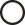
\includegraphics[scale=1]{img/Q_swap_l1.jpg}
       -- wierzchołek zwykły\newline
       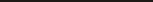
\includegraphics[scale=1]{img/Q_swap_l4.jpg}
       -- krawędź ścieżki\newline
      \end{center}
      \begin{center}
       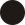
\includegraphics[scale=1]{img/Q_swap_l2.jpg}
       -- wierzchołek wadliwy\newline
       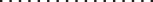
\includegraphics[scale=1]{img/Q_swap_l5.jpg}
       -- krawędź spoza ścieżki\newline
      \end{center}
      \begin{center}
       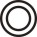
\includegraphics[scale=1]{img/Q_swap_l3.jpg}
       -- port\newline
       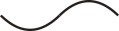
\includegraphics[scale=1]{img/Q_swap_l6.jpg}
       -- nieistotna reszta ścieżki\newline
      \end{center}
     \end{multicols}
     \noindent
     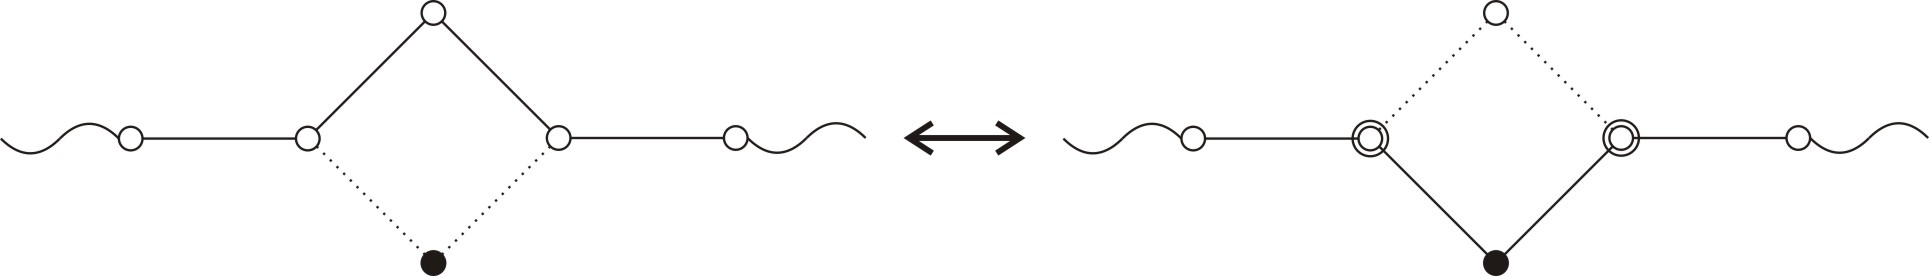
\includegraphics[scale=1]{img/Q_swap_1.jpg}\newline\newline
     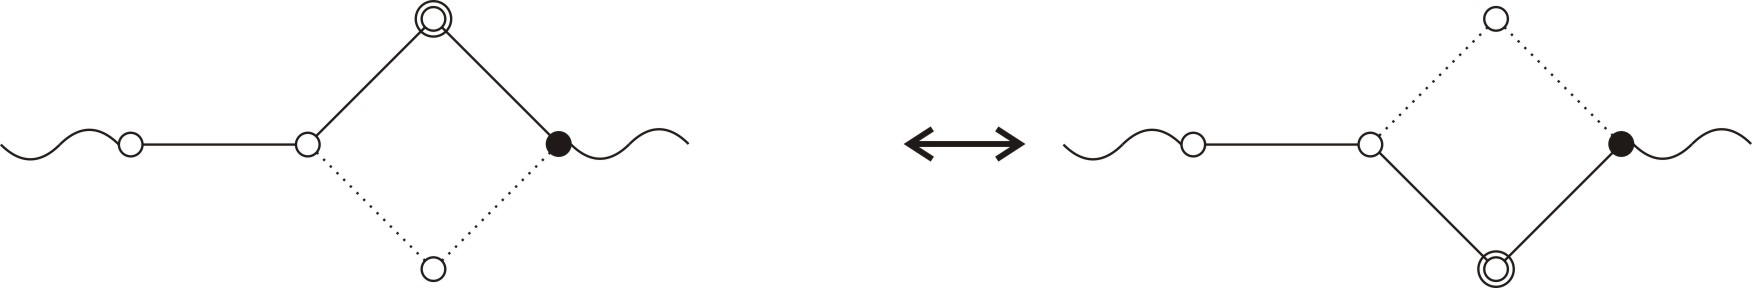
\includegraphics[scale=1]{img/Q_swap_2.jpg}\newline\newline
     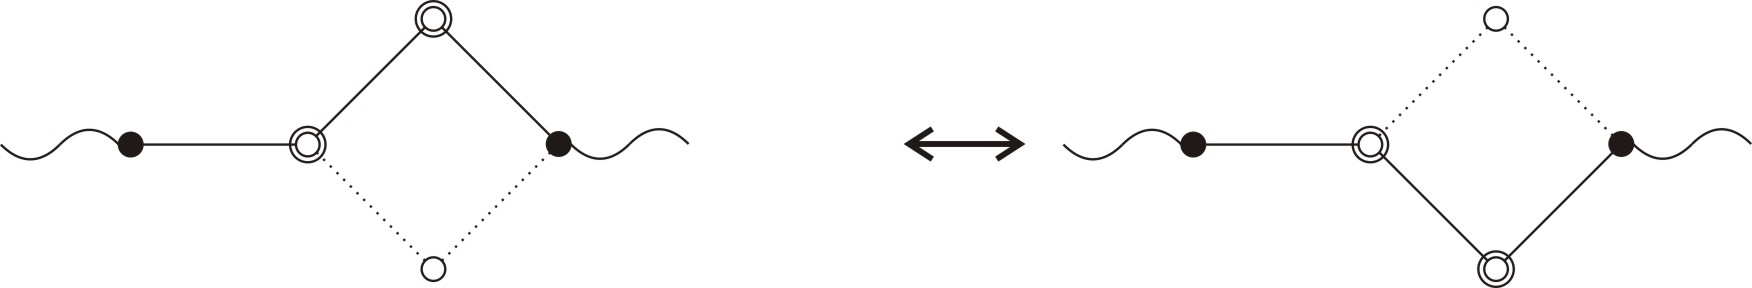
\includegraphics[scale=1]{img/Q_swap_3.jpg}\newline\newline
     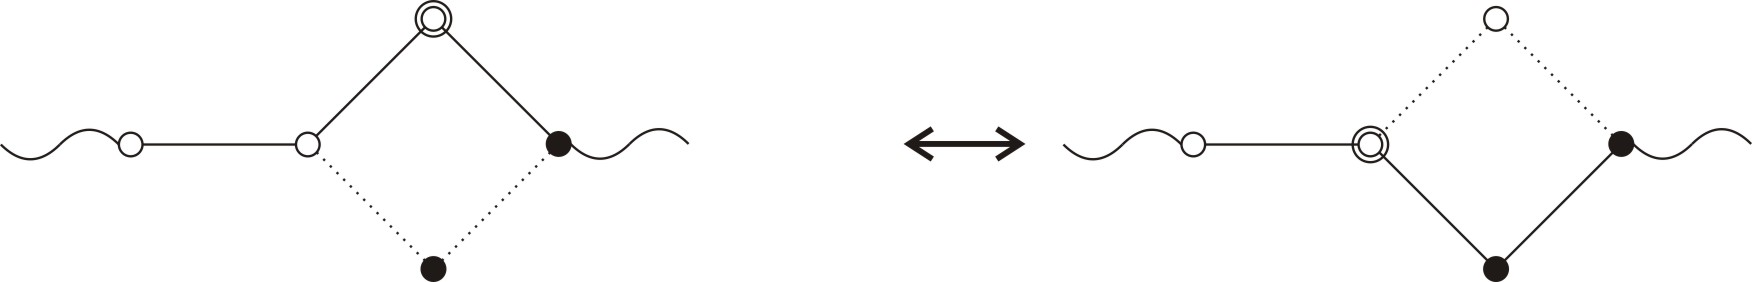
\includegraphics[scale=1]{img/Q_swap_4.jpg}\newline\newline
     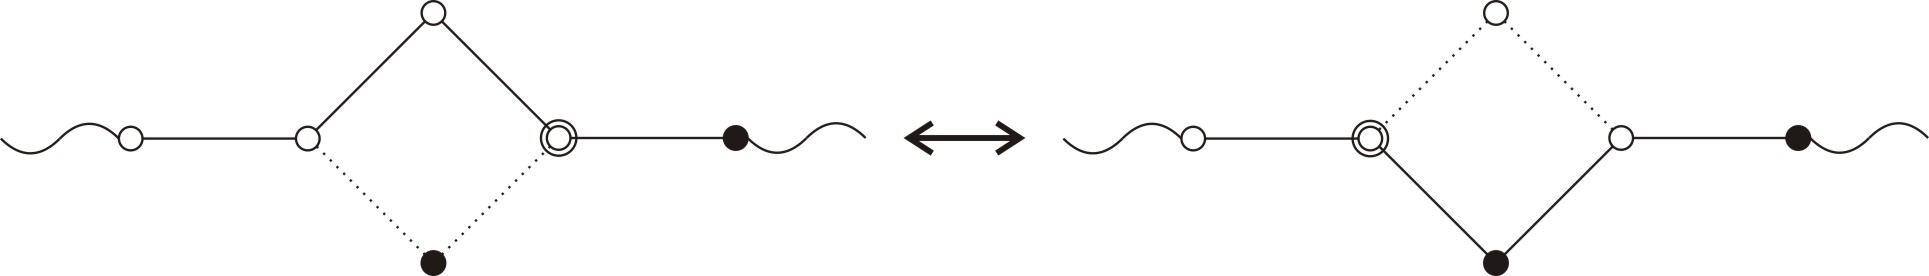
\includegraphics[scale=1]{img/Q_swap_5.jpg}\newline\newline
     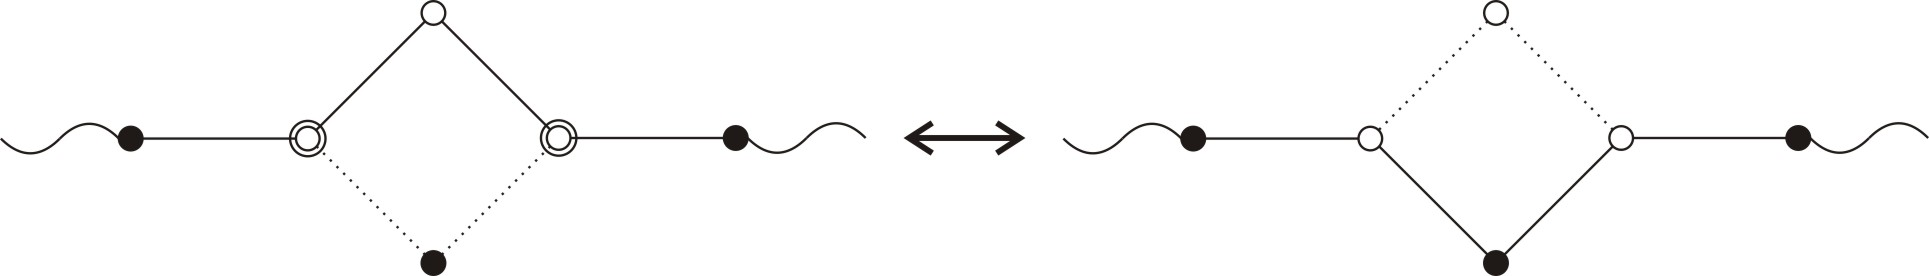
\includegraphics[scale=1]{img/Q_swap_6.jpg}\newline\newline
     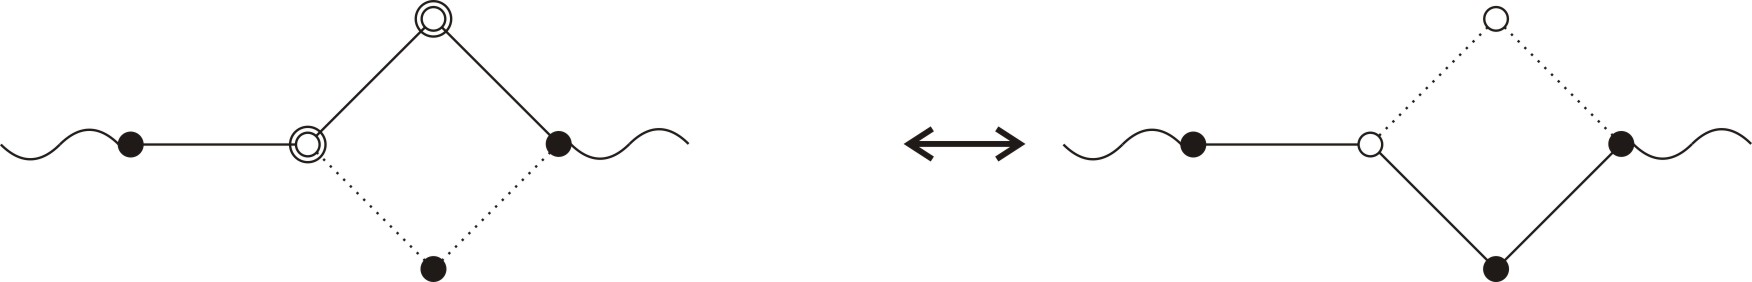
\includegraphics[scale=1]{img/Q_swap_7.jpg}\newline\newline
     Wszystkie rozrysowane tu wierzchołki należą do $G(F)$, a rozrysowane części niewadliwe tworzą podgraf spójny, dlatego też wszystkie te zmiany odbywają się w
     jednej spójnej składowej $G(F)-F$. Za każdym razem ilość portów zmienia się o $0$ lub $2$, a więc parzystość pozostaje bez zmian.
    \end{proof}
   \subsection{Dowód twierdzenia o lokalnej spójności}
    \begin{lemma}\label{Q_n-F spojne => G(F)-F spojne (1 skladowa)}
     Niech $F\subseteq V(Q_n)$ takie, że $G(F)$ jest spójne. Jeśli $Q_n-F$ jest spójne, to $G(F)-F$ również.
    \end{lemma}
    \begin{proof}
     Załóżmy przeciwnie -- istnieją wierzchołki $u,v\in A\cup B=V(G(F)-F)$ dla których istnieje ścieżka $P$ w $Q_n-F$, ale nie ma takiej w  $G(F)-F$.
     Skoro w $G(F)-F$ nie ma takiej ściezki, to w $P$ musi występować wierzchołek $x$ spoza $A\cup B$.\newline
     $G(F)$ jest spójne, więc musi istnieć też druga ścieżka $R$ łacząca $u$ z $v$ w tym właśnie grafie, na której występuje wierzchołek $y\in F$.\newline
     Podobnie jak w dowodzie lematu \ref{przeksztalcanie sciezek} 
     ścieżki te mogą być napompowane w wierzchokach $x$ i $y$ odpowidnio sekwencjami operacji $insert$.\newline
     Ponieważ $x$ jest oddalone od $F$ dodane do ścieżki $P$ wierzchołki nie uczynią z zadnego wystąpienia $x$ portu i same również nie staną się portami.
     Ponieważ $y$ należy do $F$ dodane do ścieżki $R$ wierzchołki będą miały dokładnie dwóch sąsiadów z $F$ (tego samego dwukrotnie), a więc nie będą portami.\newline
     Oznacza to, że uzyskane ścieżki równoważne mają tyle samo portów we wszystkich spójnych składowych $G(F)-F$ co odpowiadające im nieprzekształcone
     a na podstawie lematów \ref{przeksztalcanie sciezek} i \ref{parzystosc portow swap} ich parzystości między sobą się zgadzają (czyli zgadzają się dla $P$ i $R$).
     Na ścieżce $P$ nie ma żadnych portów ponieważ nie występuje w niej żaden wierzchołek wadliwy,
     daje to sprzeczność ponieważ dla spójnych składowych $G(F)-F$ w której występują
     $u$ i $v$ ścieżka $R$ ma nieparzyste ilości portów (np. można dobrać taką ścieżkę, która wchodzi do/opuszcza składowe co najwyżej raz).
    \end{proof}
    \begin{corollary}\label{Q_n-F spojne => Q_n^2[F]-F spojne (1 skladowa)}
     Dla $F\subseteq V(Q_n)$ takiego, że $Q_n^2[F]$ jest spójne ze spójności $Q_n-F$ wynika spójność $G(F)-F$.
    \end{corollary}
    \begin{proof}
     Jeśli dwa wierzchołki $Q_n^2[F]$ są połączone, to w oryginalnym grafie musiały być w odległości $\le 2$, a więc w $G(F)$ muszą być połączone
     albo bezpośrednio albo poprzez pojedynczy wierzchołek z $A$, a więc graf $G(F)$ jest spójny co sprawia,
     że spełnione są założenia lematu.
    \end{proof}
    \begin{lemma}\label{Q_n^2[F]-F spojne => Q_n-F spojne}
     Niech $F\subseteq V(Q_n)$ taki, że $G(C)-C$ jest spójne dla kazdej $C$ spójnej składowej $Q_n^2[F]$. Wtedy $Q_n-F$ również jest spójny.
    \end{lemma}
    \begin{proof}
     Dla dowolnie wybranych dwóch wierzchołków $u,v\in V(Q_n-F)$ weźmy $W$ -- ścieżkę między nimi w pełnym $Q_n$. Jeśli $W$ nie zawiera wadliwego wierzchołka,
     to jest poprawną ścieżką w $Q_n-F$. W przeciwnym przypadku znajdujemy na tej ścieżce pierwsze wystąpienie wierzchołka wadliwego.
     Poprzedni wierzchołek na ścieżce oraz pierwszy kolejny z poza zbioru $F$ są dwoma niewadliwymi wierzchołkami należącymi do $G(C)$, gdzie $C$
     jest spójną składową $Q_n^2[F]$ (oddalone o 1 od wadliwych wierzchołków, które są połączone ścieżką samych wadliwych wierzchołków).
     W $G(C)$ nie ma wadliwych wierzchołków spoza $C$, ponieważ oznaczałoby to, że taki wierzchołek jest oddalony o $\le 2$ od pewnego wierzchołka z $C$,
     a więc byłby z nim połączony w $Q_n^2$, dlatego też ścieżka ze spójnego z założenia $G(C)-C$ nie zawiera wadliwego wierzchołka.
     Wystarczy więc wadliwą część ścieżki $W$ zastąpić odpowiednią ścieżką z $G(C)-C$ aby otrzymać poprawną ścieżkę w $Q_n-F$.
    \end{proof}
    \begin{proof}
     (Twierdzenia \ref{spojnosc z lokalnej spojnosci})\newline
     Lemat \ref{Q_n^2[F]-F spojne => Q_n-F spojne} jest implikacją w jedną stronę.
     W drugą stronę dla spójnego $Q_n^2[F]$ jest dana wnioskiem \ref{Q_n-F spojne => Q_n^2[F]-F spojne (1 skladowa)}.
     Wystarczy udowodnić, że nic nie psuje się w przypadku gdy $Q_n^2[F]$ ma więcej niż jedną spójną składową.
     Dla $C$ -- spójnej składowej $Q_n^2[F]$ jeśli $Q_n-F$ jest spójne, to jest takie również $Q_n-C$
     (dla wierzchołków spoza $Q_n-F$ te same ścieżki są dobre, dla tych z  $F\backslash C$ dowolny sąsiad nalezy do $Q_n-F$, więc również łatwo zbudować ścieżkę),
     a więc spójne jest również $G(C)-C$ co kończy dowód.
    \end{proof}
   \subsection{Algorytm}
    Stosując powyższe twierdzenie można uzyskać wielomianowy algorytm uzywając jedynie przeszukiwania grafowego
    podobnie jak w podrozdziale \ref{podejscie ekspansywne}. Można jednak uzyskać lepsze rezultaty używając dodatkowo struktury $Find$--$Union$ i sprawdzając
    spójności już w trakcie budowania podgrafów $G(C)-C$.\newline
    W algorytmie używane są:
    \begin{itemize}
     \item struktura $Find$--$Union$ $D$ z operacjami:
      \begin{itemize}
       \item $Make(v,D)$ tworzącą singleton $\{v\}$
       \item $Find(v,D)$ zwracającą wskaźnik na zbiór zawierający $v$
       \item $Union(u,v,D)$ łączącą zbior zawierający $u$ ze zbiorem zawierającym $v$
      \end{itemize}
      których zamortyzowany czas można ograniczyć przez $O(log m)$ (a da się nawet uzyskać $O(log^*m)$), gdzie $m$ jest ilością użyć
      operacji $Make(v,D)$.
      Dodatkowo struktura zapewnia możliwość sprawdzenia, czy zawiera więcej niż jeden zbiór (wystarczy pojedynczy licznik inkrementowany przy
      $Make(v,D)$ i dekrementowany przy $Union(u,v,D)$).
     \item strukturę $T$ do przechowywania informacji o niektórych wierzchołkach jak binarne drzewo prefiksowe lub hashmapa,
      przechowywującą dla wierzchołka $v_T$ informacje:
      \begin{itemize}
       \item wskaźnik do wierzchołka $v$ w strukturze $D$
       \item informacje o wadliwości/braku wadliwości wierzchołka
       \item binarną informacje o tym czy wierzchołek był odwiedzony i należy do $F\cup N(F)$
      \end{itemize}
      wspierającą operacje:
      \begin{itemize}
       \item $Insert(v,T)$ wstawiającą wierzchołek $v$ do struktury $T$ i zwracającą wskaźnik na $v_T$
       \item $Retrieve(v,T)$ zwracającą $v_T$ lub $NULL$ w przypadku gdy $v$ nie ma w strukturze
      \end{itemize}
      które wymagają $O(n)$ czasu na wykonanie.
    \end{itemize}
    
    Definiuję pomocniczą funkcję uzyskiwania wierzchołków ze struktury $T$ i inicjalizowania w razie nieobecności:\newline\newline
    \hspace*{0pt}$Retrieve2(v,T)\{$\newline
    \hspace*{16pt}	$v_T=Retrieve(v,T);$\newline
    \hspace*{16pt}	if$(v_T==NULL)\{$\newline
    \hspace*{32pt}		$v_T=Insert(v,T);$\newline
    \hspace*{32pt}		$v_T.healthy=TRUE;$\newline
    \hspace*{32pt}		$v_T.visited=FALSE;$\newline
    \hspace*{32pt}		$Make(v,D);$\newline
    \hspace*{16pt}	$\}$\newline
    \hspace*{16pt}	return$(v_T);$\newline
    \hspace*{0pt}$\}$\newline
    
    Najistotniejszą częścią algorytmu jest procedura (czasami dla wielu wierzchołków z $F$) $DFS(f)$ znajdująca spójne składowe $G(C)-C$,
    dla $C$ spójnej składowej $Q_n^2[F]$ zawierającej wadliwy wierzchołek $f$, o następującym pseudokodzie:\newline\newline    
    \hspace*{0pt}$DFS(f)\{$\newline
    \hspace*{16pt}	foreach$(u\in N(f))\{$\newline
    \hspace*{32pt}		$u_T=Retrieve2(u,T);$\newline
    \hspace*{32pt}		if$(u_T.visited==FALSE)\{$\newline
    \hspace*{48pt}			$u_T.visited=TRUE;$\newline
    \hspace*{48pt}			if$(u_T.healthy)\{$\newline
    \hspace*{64pt}				foreach$(v\in N(u))\{$\newline
    \hspace*{80pt}					$v_T=Retrieve2(v,T);$\newline
    \hspace*{80pt}					if$(v_T.healthy)\{$\newline
    \hspace*{96pt}						if$(Find(u,D)\neq Find(v,D))\quad\backslash\backslash$ krawędź $uv$ należy do $G(C)-C$\newline
    \hspace*{80pt}					$\}$else if$(v_T.visited==FALSE)\{$\newline
    \hspace*{96pt}						$v_T.visited=TRUE;$\newline
    \hspace*{96pt}						$DFS(v);\quad\backslash\backslash$ wadliwy wierzchołek należący do $C$\newline
    \hspace*{80pt}					$\}$\newline
    \hspace*{64pt}				$\}$\newline
    \hspace*{48pt}			$\}$else$\quad DFS(u);\quad\backslash\backslash$ wadliwy wierzchołek należący do $C$\newline
    \hspace*{32pt}		$\}$\newline
    \hspace*{16pt}	$\}$\newline
    \hspace*{0pt}$\}$\newline
    
    Powyższa prodedura uruchamiana jest z funkcji głównej:\newline\newline
    \hspace*{0pt}$Conectivity(n,F)\{$\newline
    \hspace*{16pt}	$T=empty\_structureT();$\newline
    \hspace*{16pt}	foreach$(f\in F)\{$\newline
    \hspace*{32pt}		$f_T=Insert(f,T);$\newline
    \hspace*{32pt}		$f_T.healthy=FALSE;$\newline
    \hspace*{32pt}		$f_T.visited=FALSE;$\newline
    \hspace*{16pt}	$\}$\newline
    \hspace*{16pt}	foreach$(f\in F)\{$\newline
    \hspace*{32pt}		$f_T=Retrieve(f,T);$\newline
    \hspace*{32pt}		if$(f_T.visited==FALSE)\{$\newline
    \hspace*{48pt}			$f_T.visited=TRUE;$\newline
    \hspace*{48pt}			$D=empty\_structureD();$\newline
    \hspace*{48pt}			$DFS(f);$\newline
    \hspace*{48pt}			if$(D.counter>1)\quad return(FALSE);$\newline
    \hspace*{32pt}		$\}$\newline
    \hspace*{16pt}	$\}$\newline
    \hspace*{16pt}	return$(TRUE);$\newline
    \hspace*{0pt}$\}$
   \subsection{Analiza złożoności}
    \begin{corollary}\label{zlozonosc lokalnej spojnosci}
     Algorytm ma pesymistyczną złożoność czasową i pamięciową $O(|F|\cdot n^3)$.
    \end{corollary}
    \begin{proof}
     Dla kazdego wierzchołka z $F$ każdy sąsiad jest przeglądany po jeden raz, dla każdego wierzchołka nalezącego do $N(F)$ również przeglądani są wszyscy sąsiedzi
     po razie. Przeglądnięcie jedengo wierzchołka (znalezienie odpowiedniego wierzchołka w $T$ i $D$) zajmuje $O(n)$,
     ustawienie właściwości w $D$ zajmuje stały czas po posiadaniu dowiązania do odpowiedniego wierzchołka -- daje to złożoność tej części $O(|F|\cdot n^3)$.\newline
     Operacja $Make(v,D)$ używana jest dla każdego wierzchołka z $G(C)-C$ po razie dla kazdego $C$
     (moze być użyta więcej niż raz dla wierzchołków oddalonych o 2 od $F$ i występujących w różnych $G(C)$).
     W przypadku $Find(v,D)$ i $Union(u,v,D)$ uruchamiane są one maksymalnie odpowiednio dwa i jeden raz dla kazdego z sąsiadów wierzchołków $N(F)$
     -- daje to złożoność $O(|F|\cdot n^2\log(n))$.\newline
     Preprocessing i Postprocessing (tworzenie i usuwanie struktur $T$ i $D$)
     może być zrobione w czasie liniowym od ich wielkości (w przypadku $D$ i hashmapy można trzymać dodatkowo nieuporządkowaną listę dowiązań do wszystkich
     elementów). W przypadku struktury $T$ wielkość tą można ograniczyć przez $O(|F|\cdot n^3)$ przy użyciu drzewa prefiksowego
     (lub $O(|F|\cdot n^2)$ przy użyciu hashmapy, która nie pozwala jednak uzyskać odpowiedniej złożoności przy pesmistycznym scenariuszu),
     zaś w przypadku struktur $D$ łącznie $O(|F|\cdot n^2)$.
    \end{proof}
  \section{Wnioski i zastosowania}
   \subsection{Cykl Eulera}
    Mając dostępny efektywny algorytm badania spójności wysnułem następujący wniosek: 
 
    \begin{theorem}\label{cykl Eulera}%TODO naprawić opisy po przeniesieniu i dodać, że sam to zrobiłem
     Dla $F\subseteq V(Q_n)$ można rozstrzygnąć, czy w $Q_n-F$ jest cykl Eulera w czasie $O(|F|\cdot n^3)$
    \end{theorem}
    \begin{proof}
     Kryterium istnienia cyklu Eulera jest to, że po pierwsze graf jest spójny, a po drugie z każdego wierzchołka wychodzi parzyście wiele krawędzi.
     Spójność można sprawdzić w czasie $O(|F|\cdot n^3)$ przy pomocy algorytmu z poprzedniego podrozdziału.
     Wierzchołek nie mający wadliwego sąsiada ma stopień $n$, wystarczy więc policzyć tylko parzystość dla tych którzy takiego sąsiada mają.
     W czasie i pamięci $O(|F|\cdot n^2)$ można wstawić wszystkich niewadliwych sąsiadów wierzchołków wadliwych
     do drzewa prefiksowego zapamiętując w liściach krotność.
     Po wszystkim wystarczy dla $^2|n$ sprawdzić czy wszystkie wstawione wierzchołki mają krotność parzystą, zaś dla $^2\nmid n$ trzeba po pierwsze sprawdzić,
     że wszystkie wstawione wierzchołki mają krotność nieparzystą, a po drugie że jest ich dokładnie $2^n-|F|$.
    \end{proof}
   \subsection{Istnienie ścieżki między dwoma punktami}
    Pomimo gorszej złożoności algorytmu ekspansywnego ma on wciąż przydatne zastosowania. Jeśli nie chcemy badać spójności całego grafu, a jedynie sprawdzić
    czy istnieje w nim ścieżka między dwoma wybranymi wierzchołkami algorytm ten łatwo zredukować:
    \begin{theorem}
     Dla $F\subseteq V(Q_n)$ i dwóch wierzchołków $u,v\in Q_n-F$ można w czasie $O(n^{2.5}|F|)$ rozstrzygnąć, czy w $Q_n-F$ istnieje $uv$--ścieżka.
    \end{theorem}
    \begin{proof}
     Chcemy sprawdzić czy dwa wierzchołki należą do jednej spójnej składowej grafu $Q_n-F$. Zgodnie z lematem \ref{klasyfikacja skladowych}
     jeśli spójne składowe w których znajdują się te wierzchołki są większe niż $\frac{|F|}{\varepsilon}$, to są składową główną (a więc tą samą),
     wystarczy więc z obu wierzchołków wystartować przeszukiwanie grafowe i zakończyć je jeśi zbada się tyle wierzchołków.
     Jeśli oba wyszukiwania zakończą się dzięki temu kryterium, lub jeśli zostanie napotkany ten drugi wierzchołek, to w $Q_n-F$ istnieje $uv$--ścieżka,
     w przeciwnym przypadku nie. Tak przedstawiony algorytm działa dla dowolnego grafu (spójnego z którego usuwamy wierzchołki)
     z odpowiednią wartością $\varepsilon$. W przypadku hiperkostki wystarczy sprawdzić sąsiadów $2\sqrt{\pi n}\cdot|F|$ wierzchołków (a każdy ma ich $n$),
     podczas gdy każda taka operacja kosztuje $O(n)$, co daje koszt z twierdzenia.
    \end{proof}    
   \subsection{Długość ścieżki między dwoma punktami}
    \begin{fact}
     Dla spójnego grafu $Q_n-F$ pomiędzy każdymi dwoma wierzchołkami jest ścieżka długości nie większej niż $n+n^2\cdot|F|$.
    \end{fact}
    \begin{proof}
     Jest to bezpośredni wniosek z dowodu lematu \ref{Q_n^2[F]-F spojne => Q_n-F spojne}. Dwa dowolne wierzchołki są połączone w pełnej hiperkostce $Q_n$
     ścieżką długości co najwyżej $n$. W dowodzie zastępujemy (być może kilka razy)
     część takiej ścieżki inną ścieżką w grafie $G(C)-C$. Łącznie długość wszystkich takich zastąpień nie może wynosić więcej niż wynosi rozmiar $G(F)-F$,
     co dowodzi tezy.
    \end{proof}

 \chapter{Długie ścieżki i cykle w grafie} %TODO jeśli wyłącze podrozdziały o poziom wyżej, to trzeba zmienić wewnętrzne odniesienia typu w poprzednim podrozdziale
  W poprzednim rozdziale przedstawiony był przykład problemu na wadliwej hiperkostce, dla którego można było znaleźć rozwiązanie wielomianowe od $n$ i $|F|$.
  W tym rozdzialę przedstawię kilka problemów, dla których samo przedstawienie wyników wymagało by wykładniczej pamięci,
  jednak samo rozstrzygnięcie czy rozwiązanie istnieje (sprawdzenie warunków twierdzenia) jest możliwe w czasie
  $O(|F|\cdot n)$ dla odpowiednio małych $|F|$ (wartości podane w sformułowaniach twierdzeń).
  W przypadku podwójnych ścieżek twierdzenie daje jedynie warunek wystarczający, dlatego algorytm otrzymany dzięki niemu nawet dla tych małych $|F|$ potrafi
  jedynie rozstrzygnąć pomiędzy "istnieją długie ścieżki" i "kryterium nie rozstrzyga".
  \section{Definicje}
   \begin{defi}\label{dluga sciezka}
    Wolną od wad (nieprzechodzącą przez wierzchołki wadliwe)
    ścieżkę bez powtórzeń (drogę) w hiperkostce $Q_n$ z wadami ze zbioru $F\subseteq V(Q_n)$ nazwiemy długą, jeśli ma długość co najmniej $2^n-2|F|-2$.
   \end{defi}
   \begin{defi}\label{dlugi cykl}
    Wolny od wad cykl bez powtórzeń w hiperkostce $Q_n$ z wadami ze zbioru $F\subseteq V(Q_n)$ nazwiemy długim, jeśli ma długość co najmniej $2^n-2|F|$.
   \end{defi}
   \begin{remark}\label{dluga sciezka- nie da sie dluzszej}
    Dla $F\cup\{u,v\}$ należącego do jednej dwudzielnej części $Q_n$ nie da się skonstruować $uv$--ścieżki wolnej od wad o długości większej niż $2^n-2|F|-2$
    (stąd długośc w definicji).
   \end{remark}
   \begin{proof}
    Skoro $Q_n$ jest dwudzielna, to każda ścieżka musi odwiedzić tyle samo wierzchołków w obu częściach (plus jeden koniec), ponieważ w części z $u$ i $v$
    odwiedza co najwyżej $2^{n-1}-|F|$, to w drugiej co najwyżej $2^{n-1}-|F|-1$ -- daje to długość $2^n-2|F|-2$.
   \end{proof}
   \begin{defi}\label{wierzcholek otoczony}
    Wierzchołek $v\in V(Q_n)$ jest \emph{otoczony} przez $F\subseteq V(Q_n)$ gdy $N(v)\subseteq F$ ($F$ zawiera wszystkich sąsiadów $v$).
   \end{defi}
   \begin{defi}\label{para zablokowana}
    Dla $u,v\in V(Q_n), F\subseteq V(Q_n)$
    trójka $(u,v,F)$ jest \emph{zablokowana w $Q_n$} gdy $u$ jest otoczony przez $\{v\}\cup F$ lub $v$ jest otoczony przez $\{u\}\cup F$.
   \end{defi}
  \section{Długie ścieżki}
   \begin{theorem}\label{tw o dlugich sciezkach, male n}
    Dla $Q_n$ i $F\subseteq V(Q_n)$, takich, że $2\le n \ge 5$ i $|F|\le 2n-4$ dla $u,v\in V(Q_n)\backslash F$ takich, że trójka $(u,v,F)$
    nie jest zablokowana  w $Q_n$ długa $uv$--ścieżka bez wad nie istnieje tylko wtedy, gdy $n=4$ oraz istnieją takie $a,b\in V(Q_n)$,
    że $d(a,b)=4$  i $F\cup\{u,v,a,b\}$  jest dwudzielną częścią $Q_n$.
   \end{theorem}
   \begin{proof}%TODO może rozwinąć o ten przypadek szczególny.
    Łatwo rozpatrzyć wszystkie przypadki.
   \end{proof}
   \begin{theorem}\label{tw o dlugich sciezkach}
    Dla $Q_n$ i $F\subseteq V(Q_n)$, takich  że  $n\ge 6$ i $|F|\le 2n-4$ dla każdych $u,v\in V(Q_n)\backslash F$ jeśli $(u,v,F)$ nie jest zablokowane w $Q_n$,
    to istnieje długa $uv$--ścieżka bez wad.
   \end{theorem}
   \begin{proof}
    (krótki szkic dowodu z pracy \cite{FG})\newline
    Dowód oparty jest na indukcji po wymiarze.
    Podstawę indukcji stanowi twierdzenie \ref{tw o dlugich sciezkach, male n}.%TODO może prof. Rytter będzie wolał wyciąć ten długi fragment o 2n-6
    Dla $n\ge6$, $|F|\le 2n-4$ można podzielić $Q_n$ na dwie kostki $Q_{n-1}$ wybierając jedną z $n$ współrzędnych 
    i definiując podkostki $Q^0_{n-1}$ i $Q^1_{n-1}$ jako rozpięte przez wierzchołki mające na tej współrzędnej odpowiednio $0$ i $1$.
    Dla $|F|\le 2n-5$ łatwo jest dobrać współrzędną tak, żeby każda z podkostek miała co najwyżyżej $2n-6=2(n-1)-4$ wadliwych wierzchołków
    (wystarczy wybrać dowolne $f_1,f_2\in F$ i podzielić według jednej ze współrzędnych różniących ich ciągi binarne).
    Dla $|F|=2n-4$ można rozpatrzyć macierz $|F|\times n$, w której w wierszach wypisane są ciągi binarne wszystkich wierzchołków wadliwych.
    Trzeba wybrać taką kolumnę, w której zarówno $0$ jak i $1$ jest co najmmniej po 2. Gdyby nie dało się dokonać takiego wyboru oznaczało by to, że
    w każdej kolumnie jest albo co najwyżej jedno $0$ albo co najwyżej jedna $1$, przez proste zanegowanie jednej współrzędnej w całej kostce
    (ta operacja nie zmienia nic poza numerowaniem) można uzyskać przypadek, że w każdej kolumnie jest co najwyżej jedna $1$. 
    Ponieważ kolumn jest tylko $n$, zaś każda zawiera co najwyżej jedną $1$, to oznaczało by to, że może mieć tylko $n+1$ różnych wierszy
    $\Rightarrow 2n-4=|F|\le n+1\Rightarrow n\le5$ (a więc ponieważ $n\ge 6$, to zawsze istnieje wybór współrzędnej).\newline
    Dalej przy użyciu lematów:
    \begin{itemize}
     \item Dla $|F|\le 2n-3$ co najwyżej jeden z wierzchołków jest otoczony przez $F$.
     \item Dla $|F|\le 2n-4$ i ustalonego nieotoczonego wierzchołka $u$ istnieje co najwyżej jeden wierzchołke $v$ taki, że $(u,v,F)$ jest zablokowana.
     \item Dla $|F|\le 2n-5$ tylko jedna trójka $(u,v,F)$ moze być zablokowana, i to taka, że $uv\in E(Q_n-F)$.
    \end{itemize}
    i wykorzystując fakt, że w podkostkach poza kilkoma przypadkami istnieją odpowiednie długie kostki rozważa się dużą liczbę przypadków
    (rozbicie ze względu na należenie $u$ i $v$ do tej samej/różnej podkostki, bycia otoczonym/zablokowanym/wolnym w podkostce).
    Dla kazdego z tych przypadków da się pokazać metodę łączenia długich ścieżek z podkostek.
   \end{proof}
   \begin{remark}\label{dluga sciezka 2n-3 za duzo}
    Dla $Q_n$, $F\subseteq V(Q_n)$, $|F|=2n-3$ teza twierdzenia \ref{tw o dlugich sciezkach} przestaje być prawdziwa.
   \end{remark}
   \begin{proof}
   Dla każdego $n\ge 4$ istnieje po kilka przypadków w których $|F|=2n-3$, $(u,v,F)$ nie jest zablokowane, ale nie ma długiej $uv$--ścieżki bez wad.
   3 przykłady :\newline
   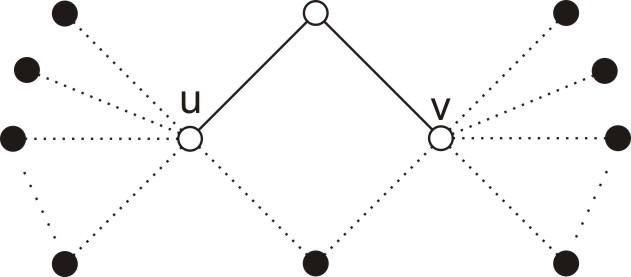
\includegraphics{img/Q_niezablokowane_1.jpg}\quad\quad\quad
   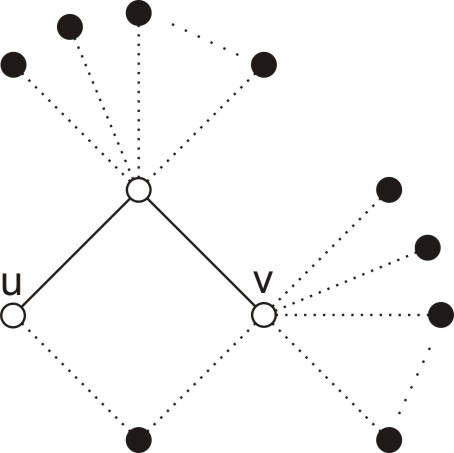
\includegraphics{img/Q_niezablokowane_2.jpg}\quad\quad\quad
   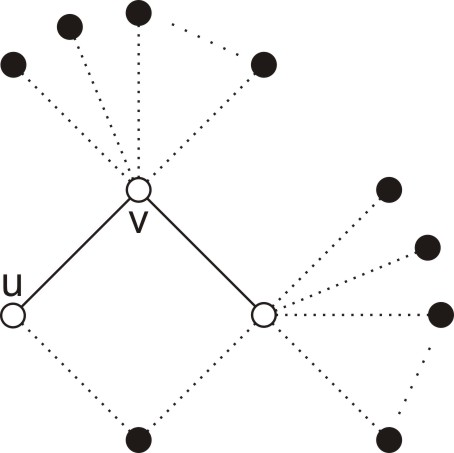
\includegraphics{img/Q_niezablokowane_3.jpg}
   \end{proof}
  \section{Długie cykle}
   \begin{defi}\label{przekrój kostki}
    Dla zbioru $D\subseteq[n], d=|D|$ oraz $u\in\{0,1\}^{n-d}$ definiujemy kostkę $Q_D(u)$ jako $d$ wymiarową podkostkę $Q_n$, której współrzędne spoza $D$
    są ustalone przez wektor $u$. Definiujemy również $V_D(u)=\{(u,v)_D:v\in\{0,1\}^d\}$ (wierzchołki z oryginalnej kostki wzięte do $Q_D(u)$), oraz
    $F_D(u)=F\cap V_D(u)$.
   \end{defi}
   \begin{lemma}\label{dlugi cykl - podzial kostki}
    Niech $F\subseteq V(Q_n)$ takie, że $|F|\ge 2n$ i niech $d=\lceil\frac{n^2}{2|F|-n-2}\rceil$.
    Wtedy istnieje zbiór $D\subseteq[n],|D|=d$, taki że $|F_D(u)|\le d+1$ dla kazdego $u\in\{0,1\}^{n-d}$
   \end{lemma}
   Lemat pochodzi z pracy \cite{Wie} i został zmodyfikowany do tej postaci w pracy \cite{FG} aby lepiej pasować do dowodu poniższego twierdzenia.
   \begin{theorem}\label{dlugi cykl - tw}
    Dla $n\ge15$ i $F\subseteq V(Q_n)$, takiego że $|F|\le\frac{n^2}{10}+\frac{n}{2}+1$ istnieje długi cykl bez wad.
   \end{theorem}
   \begin{proof}
    (krótki szkic dowodu z pracy \cite{FG})\newline
    Na podstawie lematu \ref{dlugi cykl - podzial kostki} znajdujemy zbiór $D\subseteq[n]$, taki że $|F_D(u)|\le 2d-4$ dla każdego $u\in\{0,1\}^{n-d}$.
    Dla dowolnego cyklu Hamiltona $(u_0,u_1,...,u_{2^{n-d}}=u_0)$ w $Q_{n-d}$ dobieramy w kostce $Q_D{u_i}$ dwa nie wadliwe
    wierzchołki $a_i$ oraz $b_i$, takie że $a_ib_{i+1}\in E(Q_n)$ dla kazdego $i\in[2^{n-d}]$ (modulo $2^{n-d}$),
    oraz $(a_i,b_i,F_D(u^i))$ nie zablokowane (choć jest to nietrywialne to da sie takie dobrać).
    Na podstawie twierdzenia \ref{tw o dlugich sciezkach} wierzchołki $a_i$ i $b_i$ są łączone długimi ścieżkami dając cykl długości $\ge 2^n-2|F|$.
    Ograniczenie $|F|\le\frac{n^2}{10}+\frac{n}{2}+1$ potrzebne jest po to, aby $\lceil\frac{n^2}{2|F|-n-2}\rceil\ge5$ omijając złe przypadki z twierdzenia
    \ref{tw o dlugich sciezkach, male n}.
   \end{proof}
  \section{Długie pary ścieżek}
   \begin{lemma}\label{zawsze dlugie sciezki}
    Dla $n\ge2$, $F\subseteq V(Q_n)$, $|F|\le n-2$ dla każdych dwóch $u,v\in V(Q_n-F)$ istnieje długa $uv$--ścieżka bez wad.
   \end{lemma}
   \begin{proof}
    Bezpośrednio z \ref{tw o dlugich sciezkach}, gdzie ze względu na rozmiar $F$ trójka $(u,v,F)$ nie może być zablokowana.
   \end{proof}
   \begin{theorem}\label{pary sciezek}
    Dla $F\subseteq V(Q_n)$, $F\le n-3$ niech $A$ i $B$ będą różnymi dwuelementowymi pozdbiorami $V(Q_n)-F$, takimi że $A\cup B$ nie należy do
    jednej części dwudzielnej kostki. Wtedy istnieje para wierzchołkowo rozłącznych
    ścieżek o łącznej długości $\ge 2^n-2|F|-3$ zaczynających się w wierzchołku z $A$ i kończących na wierzchołku z $B$.
   \end{theorem}
   \begin{proof}
   (krótki szkic dowodu z pracy \cite{FG2})\newline
    Dowód podobnie jak inne przebiega indukcyjnie -- małe przypadki ($n\le 5$) można sprawdzić ręcznie (tutaj trochę więcej sprawdzania niż w poprzednich dowodach),
    dla większych łatwo jest podzielić $Q_n$ na dwie $Q_{n-1}$ tak, zeby każda z nich miała nie więcej niż $n-4$ wierzchołków wadliwych.
    Dalej rozpatrywane jest dużo przypadków w zależności od podziału wierzchołków z $A$ i $B$ na dwie podkostki i w każdym z możliwych przypadków łączy się
    podwójne i pojedyncze ścieżki istniejące na mocy indukcji i twierdzenia \ref{tw o dlugich sciezkach}.
   \end{proof}
   \begin{remark}\label{a cap B=(u)}
    Jeśli $A=\{u,w\}, B=\{v,w\}$, to jedna ze ścieżek musi mieć długość $0$ i być zaczepiona w wierzchołku $w$.
    Twierdzenie \ref{pary sciezek} daje wtedy $uv$-ścieżkę
    wolną od wad długości $2^n-2|F|-3=2^n-2|F\cup\{w\}|-1$, a więc o jeden dłuższą niż w twierdzeniu \ref{tw o dlugich sciezkach}
    (możliwe jest to tylko dlatego, że $u$ i $v$ nie należą do jednej części dwudzielnej $Q_n$).
   \end{remark}
   
 \chapter{Ścieżka i cykl Hamiltona}
  \section{Kostka bez wadliwych wierzchołków}
   Pełna kostka $Q_n$ ($n\ge2$) jest grafem hamiltonowskim (posiadającym cykl Hamiltona)
   -- bardzo wiele różnych cykli Hamiltona można uzyskać już łącząc dwa cykle
   z podkostek $Q_{n-1}$ (wystarczy, że w dwóch takich cyklach jest taka sama krawędź).
   %TODO łączna ilość cykli%
   Cykle hamiltona na hiperkostce mają również zastosowania praktyczne. Jednym z przykładów użycia takich cykli są kody Graya
   -- ciągi wektorów binarnych określonej długości, które zawierają wyszytkie takie wektory, oraz posiadają tą własność,
   że dwa sąsiednie wektory różnią się tylko na jednej pozycji. Kody te znajdują zastosowanie między innymi przy minimalizacji kodowania i obwodów binarnych,
   oraz w algorytmach genetycznych i kodach korekcyjnych.\newline
   Pojawia się pytanie, czy po usunięciu kilku wierzchołków nadal da się zbudować takie cykle lub chociaż ścieżki Hamiltona.
  \section{Ogólne podejście do problemu}
   W przypadku ogólnym sprawdzenie, czy graf posiada cykl Hamiltona jest problemem NP--zupełnym, dlatego przy dowolnym wyborze zbioru wierzchołków usuniętych
   ciężko spodziewać się algorytmu w czasie $O(2^n)$, a co dopiero w $O(n^c)$. Jeśli jednak zbiór usuniętych wierzchołków
   jest odpowiednio mały lub tworzy graf z jakiejś wąskiej klasy, to istnieją dowody istnienia takiego cyklu.
   
   \begin{defi}\label{graf zbalansowany}
    Graf dwudzielny nazywamy \emph{zbalansowanym} jeśli jego dwie części dwudzielne mają ten sam rozmiar,
    zaś \emph{prawie zbalansowanym} jeśli ich rozmiary różnią się o 1.
   \end{defi}    
   
   Hiperkostka jest grafem dwudzielnym, więc i po usunięciu części wierzchołków takim pozostanie,
   jako że dowolny cykl w takim grafie odwiedza tyle samo wierzchołków w obu częściach dwudzielnych (z krotnościami),
   to podstawowym warunkiem koniecznym jest to, żeby z obu tych części usunąć dokładnie tyle samo wierzchołków.
   W przypadku ścieżki Hamiltona koniecznym jest żeby graf był zbalansowany lub prawie zbalansowany.
   
   \begin{defi}\label{Hamiltonian lacable}%TODO
    Graf dwudzielny (z częściami $U$ i $v$) nazywamy hamiltonowsko wiązalnym jeśli:
    \begin{itemize}
     \item jest zbalansowany i dla każdej pary $u\in U,v\in V$ istnieje ścieżka Hamiltona z $u$ do $v$.
     \item jest prawie zbalansowany i dla każdej pary $u,u'\in U$ (gdzie $U$ to ta większ składowa) istniała ścieżka Hamiltona
      z $u$ do $v$.
    \end{itemize}
   \end{defi}
   Jeśli graf jest zbalansowany i hamiltonowsko wiązalny, to istnieje w nim cykl Hamiltona (jeśli ma więcej niż 2 wierzchołki).\newline
   Hiperkostka jest grafem hamiltonowsko wiązalnym.\newline

   W 2001 Stephen Locke postawił hipotezę:
   \begin{conjecture}\label{Locke conjecture}
    Niech $F\subseteq V(Q_n)$ będzie zbiorem po $k$ wierzchołków z obu dwudzielnych składowych $Q_n$. Wtedy $Q_n-F$ posiada cykl hamiltona jeśli
    $n\ge k+2$.
   \end{conjecture}
   Od tego czasu udowodnione zostały szczególne przypadki tej hipotezy ($k\le3$, $k\le\frac{n-5}{6}$,...),
   a w 2009 podane zostało ich uzupełnienie -- dowód indukcyjny po $n$ w pracy \cite{Locke}, który jednak po kilka przypadków granicznych odsyła
   do drugiej pracy, którą autorzy mają dopiero opublikować.
   
  \section{Dowody dla szczególnych przypadków F}
   \begin{defi}\label{podgraf izometryczny}
    Podgraf H grafu G nazywamy \emph{izometrycznym} jeśli $d_H(u,v)=d_G(u,v)$ dla każdych $u,v\in V(H)$.
   \end{defi}
   Łatwo zauważyć, że podgraf izometryczny jest zawsze podgrafem indukowanym przez podzbiór wierzchołków,
   implikacja w drugą stronę jednak nie zachodzi (na przykład $P_4$ jako podgraf $C_5$).
   \subsection{podkostka}
    \begin{fact}\label{hamilton dla F=Q_m}
     Jeśli jako $F\subseteq V(Q_n)$, $n\ge3$ weźmiemy zbiór wierzchołków podkostki $Q_m$ ($1\le m<n$), to $Q_n-F$ posiada cykl Hamiltona.
    \end{fact}
    \begin{proof}
     Dla $m\ge2$:\newline 
     Porządany cykl Hamiltona w $Q_n-F$ można otrzymać poprzez podział grafu na $2^{n-m}-1$ kostek $Q_m$, wybranie tego samego cyklu Hamiltona dla tych podkostek
     a następnie połączenie ich w następujący sposób:\newline
     Wybieramy jedną z podkostek, która wraz z usuniętą tworzy kostkę $Q_{m+1}$ -- taka kostka różni się od poprzedniej na dokładnie jednej współrzędnej
     (takiej która jest stała na całej podkostce). Łączymy obie i otrzymujemy w ten sposób wadiwą kostkę $Q_{m+1}$ z cyklem Hamiltona.
     Pozostałe kostki łączymy parami, razem z cyklami (wystarczy wybrać taką samą krawędź w obu i dokonać "przepięcia") -- wszystkie tak samo.
     Cykl z wadliwej hiperkostki ma tylko jedną krawędź, której nie ma w innych cyklach -- można dokonać połączenia wadliwej $Q_{m+1}$ z całą i dalej aż
     do otrzymania $Q_n-F$ z cyklem Hamiltona.\newline
     Dla $m=1$ postępujemy analogicznie, jednak po pierwszym kroku otrzymana $Q_2-Q_1$ nie ma cyklu a jedynie ścieżkę Hamiltona, jednak dalej $Q_3-Q_1$
     posiada już cykl Hamiltona, który można przedłużyć na cykl Hamiltona na $Q_3$ zawierający tę krawędź z $Q_2-Q_1$. Dalej można postępować już tak samo
     -- zawsze da się wybrać krawędź według której można dokonać "przepięcia".
    \end{proof}
    Podobnym sposobem można otrzymać cykle dla $F$ równemu sumie kilku kostek ($m\ge2$), które nie są połączone (tak długo, jak jest ich na tyle mało,
    aby dało się wybierać krawędzie do "przepięcia" -- to da się sprawdzić algorytmem wielomianowym od $n$ i $F$).\newline
   
   Poniżej przedstawię szkice dowodów twierdzeń dla innych szczególnych przypadków $F$ opisanych w pracy \cite{Pegr}.
   Ze względu na liczność mało istotnie różniących się przypadków po obrazki i dokładne opisy wyborów wierzchołków,
   które łączymy ścieżkami Hamiltona w podkostkach odsyłam to tejże pracy.
   \subsection{Ścieżka izometryczna}
    \begin{fact}\label{sciezka izo - rozne kierunki}
     W ścieżce izometrycznej w $Q_n$ każda z krawdzi ma inny kierunek, a więc ścieżka taka może mieć długość co najwyżej $n$.
    \end{fact}
    \begin{proof}
     Gdyby dwie krawędzie miały ten sam kierunek, to wierzchołki z początku pierwszej i końca drugiej można w $Q_n$ połączyć ścieżką o 2
     (przesunięta ścieżka spomiędzy tych dwóch krawędzi).
    \end{proof}
    \begin{theorem}\label{hamilton - sciezka, nieparz} %TODO zamienić graf rozpinany przez zbiór wierzchołków, na graf indukowany -- w innych miejscach pracy
     Dla $F\subseteq V(Q_n)$ indukujacego ścieżkę izometryczną nieparzystej długości $Q_n-F$ jest hamiltonowsko wiązalna jeśli $n\ge4$.
    \end{theorem}
    \begin{proof}
     Przypadek ścieżki długości $1$ indukcyjnie po $n$ -- dzielimy kostkę na dwie w kierunku $i$ -- innym niż ten krawędzi ścieżki usuniętej.
     Jedna podkostka jest pełna, zaś w drugiej jest usunięta ścieżka. Jeśli wierzchołki $u$ i $v$ tóre chcemy połączyć należą do tej samej
     podkostki, to łączymy je ścieżką Hamiltona w tej części na podstawie indukcji. Wybieramy dwa kolejne wierzchołki na tej ścieżce,
     nie będące w $Q_n$ sąsiadami $F$ w kierunku $i$, i łączymy w drugiej części ścieżką Hamiltona ich sąsiadów w tym kierunku.\newline
     Jeśli dwa wierzchołki są w różnych częściach, wystarczy wybrać dowolną parę wierzchołków, takich że: są sąsiadami w kierunku $i$, są rózne od
     $u$ i $v$, oraz należą do innych dwuspójnych składowych niż wierzchołek $u$ lub $v$ z ich części
     -- można wtedy znaleźć ścieżki Hamiltona w obu częściach pomiędzy wierzchołkami $u$ i $v$ oraz tymi wybranymi i je połączyć.\newline
     
     Dla ścieżki większej długości dzielimy hiperkostkę na dwie względem kierunku drugiej krawędzi na ścieżcę. W każdej podkostce znajduje się część ścieżki,
     która jest izometryczną nieparzystą ścieżką. Ścieżkę Hamiltona uzyskujemy jak poprzednio -- przy rozbiciu na dwa przypadkii łączeniu ścieżek z podkostek.
     Przypadek $n=4$ jest natomiast rozważany ręcznie
     (tam są możliwe tylko 2 takie ścieżki z dokładnością do zmiany wierzchołka początkowego i permutacji współrzędnych).
    \end{proof}
    \begin{theorem}\label{hamilton - sciezka, parz}
     Dla $F\subseteq V(Q_n)$ indukujacego ścieżkę izometryczną parzystej długości ($\ge2$) $Q_n-F$ jest hamiltonowsko wiązalna jeśli $n\ge5$.
    \end{theorem}
    \begin{proof}
     Ponownie indukcynie po $n$, tym razem dzieląc kostkę w kierunku pierwszej krawędzi ścieżki -- zostawiając w pierwszej podkostce pojedynczy wadliwy wierzchołek,
     zaś w drugiej kostce wymiaru $\ge4$ wadliwą ścieżkę nieparzystej długości (przypadek z poprzedniego twierdzenia).
     Tym razem należy rozpatrzyć 3 przypadki (gdy $u$ i $u'$ są w różnych kostkach i 2 przypadki, gdy są w tej samej).
     Dla każdego z tych przypadków ponownie łatwo wybrać odpowiednie ścieżki w podkostkach i połączyć je tak aby uzyskać ścieżki Hamiltonowskie w
     $Q_n-F$ od $u$ do $u'$ (szczegóły z obrazkami można zobaczyć w pracy \cite{Pegr}).
    \end{proof}
    \begin{remark}
     Na podstawie \cite{SCJY} prawdziwe jest mocniejsze stwierdzenie:\newline
     Niech $P$ będzie ścieżką w długości $\le 2n-4$ w grafie $Q_n$, wtedy $Q_n-P$ jest hamiltonowsko wiązalna.
    \end{remark}
   \subsection{Cykl izometryczny}
    \begin{remark}\label{cykl izometryczny - drugie pol powtorka}
     W cyklu izometrycznym na hiperkostce każdy kierunek krawędzi występuje dokładnie 2 razy, w antypodycznych krawędziach cyklu.
    \end{remark}
    \begin{proof}
     Każdy kierunek krawędzi musi się pojawić na dowolnym cyklu w hiperkostce parzystą ilość razy. Dla cyklu długości $2k$
     weźmy dwa wystąpienia tego samego kierunku, oddalone od siebie na cyklu o minimalną liczbę krawędzi. Dostajemy ścieżkę długości $l$ zaczynającą
     i kończącą się krawędzią tego samego kierunku. Podobnie jak w dowodzie faktu \ref{sciezka izo - rozne kierunki} mamy w hiperkostce
     inną ścieżkę długości $l-2$ łączącą te same końce. Z izometryczności $l-2\ge min(l,2k-l)$, zaś z minimalności $l-2\le 2k-l\Rightarrow l-1=k$.
    \end{proof}
    \begin{theorem}\label{hamilton - cykl, parz}
     Niech $C$ będzie izometrycznym cyklem w $Q_n$ ($n\ge6$), o długości $2k$ podzielnej przez $4$, wtedy $Q_n-P$ jest hamiltonowsko wiązalna.
    \end{theorem}
    \begin{proof}
     Zaczynamy od podzielenia hiperkostki na dwie w kierunku wyznaczonym przez pierwszą (dolowlnie wybraną) krawędź cyklu.
     W obu kostkach znajduje się wadliwa izometryczna ścieżka długości nieparzystej, a więc z tiwerdzenia \ref{hamilton - sciezka, nieparz}
     obie są hamiltonowsko wiązalne. Podobnie jak wcześniej wystarczy rozważyć dwa przypadki. Jeśli dwa wierzchołki $u$ i $v$
     które chcemy połączyć ścieżką Hamiltona należą do różnych podkostek,
     to wystarczy dobrać po jednym wierzchołku z podkostek, tak żeby te wierzchołki były sąsiadami, były różne od $u$ i $v$ i należały do odpowiednich
     części dwuspójnych -- tworzymy ścieżki w podkostkach i łączymy je ze sobą. Jeśli zaś $u$ i $v$ należą do tej samej podkostki,
     to wystarczy na ścieżce Hamiltona pomiędzy nimi wybrać dowolną krawędź, taką że sąsiedzi jej końców z drugiej hiperkostki nie są wadliwi --
     pomiędzy tymi sąsiadami wyznaczamy ścieżkę w drugiej podkostce i "dopinamy" do ścieżki z pierwszej podkostki.
    \end{proof}
   \subsection{Drzewo izometryczne}
    \begin{remark}\label{drzewo izo - kierunek tylko raz}
     W drzewie izometrycznym w $Q_n$ każda z krawędzi ma inny kierunek.
    \end{remark}
    \begin{proof}
     W przeciwnym przypadku istnieją dwie krawędzie o tym samym kierunku -- w drzewie jest ściężka, która zawiera obie krawędzie, co daje sprzeczność z lematem
     \ref{sciezka izo - rozne kierunki} (w drzewie każde dwa wierzchołki są połączone tylko jedną ścieżką, więc nie ma innej krótszej).
    \end{proof}
    \begin{remark}\label{drzewo izo zbal - ma liść z V}
     W niepustym drzewie zbalansowanym, lub prawie zbalansowanym z przewagą w części dwudzielnej $V$ jest liść zawarty w tej składowej.
    \end{remark}
    \begin{proof}
     Nie wprost -- jeśli w drzewie każdy liść należy do dwudzielnej części $U$, to można wybrać dowolny wierzchołek z $v\in V$ jako korzeń.
     Usunięcie dowolnej gałęzi bez rozwidleń (od ostatniego rozwidlenia do liścia) nie produkuje nowych liści, może też pogorszyć balans jedynie
     zwiększając przewagę $V$. Gdy zostanie już tylko jedna ścieżka, to kończyć się ona będzie z obu stron wierzchołkami z $U$, co daje sprzeczność.
    \end{proof}
    \begin{lemma}\label{Q_5-izo tree hamilton}
     Dla zbalansowanego drzewa $T$ izometrycznego w $Q_5$ graf $Q_5-T$ jest hamiltonowsko wiązalny.
    \end{lemma}
    Lemat można sprawdzić ręcznie lub komputerowo (są tylko dwa takie drzewa nie będące ścieżkami z dokładnością do umiejscowienia w kostce).
    \begin{theorem}\label{Hamilton - drzewo izo}
     Dla $T$ zbalansowanego lub prawie zbalansowanego drzewa izometrycznego w $Q_n$ graf $Q_n-T$ jest hamiltonowsko wiązalny dla $n\ge5$
     (w przypadku zbalansowanego wystarczy $n\ge4$).
    \end{theorem}
    \begin{proof}
     Dowód przez indukcję po rozmiarze hiperkostki. Jako krok bazowy można traktować lemat \ref{Q_5-izo tree hamilton}, przypadek drzewa prawie zbalansowanego
     (w $Q_5$ istnieje takie tylko jedno nie będące ścieżką) i zbalansowanego dla $n=4$ (tu są tylko ścieżki) można rozpatrzyć analogicznie dla tamtego przypadku.
     W kroku indukcyjnym dla drzewa zbalansowanego korzystamy z wymiaru o $1$ mniejszego i drzewa prawie zbalansowanego 
     zaś dla drzewa prawie zbalansowanego korzystamy z poprzedniego kroku dla drzewa zbalansowanego.
     Dla drzewa prawie zbalansowanego na podstawie uwagi \ref{drzewo izo zbal - ma liść z V} wybieramy liść
     z części dwudzielnej w której ma ono więcej wierzchołków i dzielimy hiperkostkę na dwie mniejsze według kierunku krawędzi drzewa
     wchodzącej do tego wierzchołka. Otrzymujemy w ten sposób w jednej podkostce pojedynczy wadliwy wierzchołek (jak w dowodach poprzednich twierdzeń)
     oraz w drugiej drzewo izometryczne zbalansowane. Jak we wcześniejszych dowodach w zależności od tego w których podkostkach znajdują się wierzchołki
     które chcemy połączyć ścieżką Hamiltona tworzymy ścieżki w podkostkach i łączymy je. Dla drzewa zbalansowanego postępujemy analogicznie z tą różnicą,
     że wybór liścia jest dowolny.
    \end{proof}

  \chapter{Największa odległość grafowa}%TODO sprawdzić czy zawsze nazywam tak samo współrzędne (od 0 do n-1), w innych podrozdziałach też
   \begin{defi}\label{srednica grafu}
    \emph{Średnicą grafu} nazywamy największą odległość pomiędzy jego dwoma wierzchołkami $d(G)=\max\limits_{u,v\in V(G)}d(u,v)$.
   \end{defi}
   Jedną z najważniejszych zalet hiperkostki $Q_n$, jest to, że pomimo względnie niskiej gęstości jej średnica jest niewielka i równa $n$,
   a do tego po usunięciu części węzłów często pozostaje spójna.
   Graf ten posiada również tę przyjemną własność, że przy losowym usuwaniu wierzchołków odległości pomiędzy nieusuniętymi wierzchołkami rzadko się zwiększają
   (w szczególności dla wierzchołków bardziej oddalonych).
   Przy intencjonalnym usuwaniu aby zwiększyć odległość pomiędzy dowolnymi dwoma wierzchołkami potrzeba usunąć co najmniej dwa wierzchołki
   (w przypadku dowolnych wierzhcołków oddalonych o 2), zaś aby zwiększyć średnicę grafu należy usunąć co najmniej $n-1$ wierzchołków
   (wszystkich prócz jednego sąsiadów dowolnie wybranego wierzchołka).
   Aby uzyskać średnicę $n+2$ należy usunąć $2n-3$ wierzchołków
   (na przykład sąsiedzi wierzchołków numer $1$ i $2$ oprócz $4$ i siebie nawzajem przy numerowaniu klasycznym),
   dalej jednak pojawia się coraz więcej możliwości usuwania wierzchołków i ciężko wybrać najlepszą.
    
   Zainspirowany tym postawiłem sobie pytanie jaką największą średnicę można uzyskać w ten sposób pozostawiając graf spójnym.
   Średnicę spójnego grafu $Q_n-F$ wyznacza najkrótsza ścieżka między pewnymi dwoma wierzchołkami, jeśli więc dla jakiegoś grafu uda się uzyskać
   taką maksymalną średnicę, to można wybrać tę ścieżkę i odrzucić wszystkie wierzchołki spoza niej (nie zmniejszając średnicy).
   Oznacza, to że to maksimum po wszystkich grafach $Q_n-F$ jest uzyskiwane dla grafu będącego ścieżką.
   Ścieżka taka ma tę własność, że ciągi binarne sąsiadujących w niej wierzchołków różnią się na dokładnie jednej pozycji,
   natomiast dla dowolnych dwóch nie będących sąsiadami ciągi te muszą się różnić na co najmniej dwóch pozycjach.
   Wyjściowy problem został więc zredukowany (okazał się równoważny) do problemu:\newline
   Znajdź najdłuższy ciąg wektorów binarnych długości $n$,
   że każde dwa sąsiednie wektory różnią się na co najmniej jednej pozycji, zaś każde dwa inne na co najmniej dwóch.
   \section{Ścieżka Fibonacciego}
    \begin{theorem}\label{co najmniej fibo}
     Dla danego $n$ istnieje prosty algorytm konstruujący ciąg wektorów reprezentujący ścieżkę długości $F_{n+1}$,
     (gdzie $F_n$ to $n$-ty wyraz ciągu Fibonacciego: $F_0=F_1=1$), która jest podgrafem indukowanym hiperkostki.
     Co więcej prefiks długości $F_{n}$ jest takim ciągiem dla $n-1$ (po odrzuceniu ostatniej współrzędnej wektorów).
    \end{theorem}
    \begin{proof}%TODO nazywam ścieżkę P_n - a to oznaczenie ścieżki o długości n
     Na potrzeby dowodu nazwę taką ścieżkę $P_n$.
     Dowód tradycyjnie przez indukcję po wymiarze -- dla $n\in\{0,1,2,3,4\}$ konstrukcja jest widoczna na rysunkach:\newline
     \hspace*{0pt}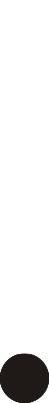
\includegraphics[scale=0.6]{img/Q0_long_path.jpg}
     \hspace*{12pt}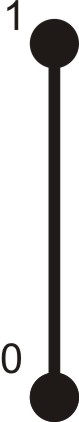
\includegraphics[scale=0.6]{img/Q1_long_path.jpg}
     \hspace*{12pt}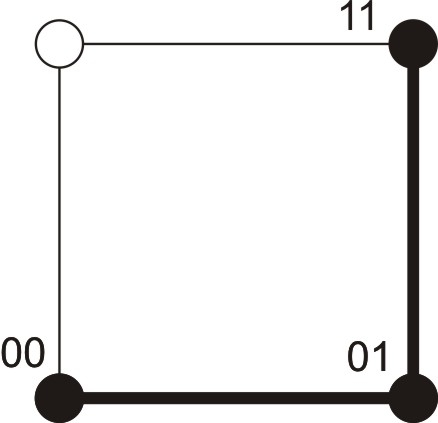
\includegraphics[scale=0.6]{img/Q2_long_path.jpg}
     \hspace*{12pt}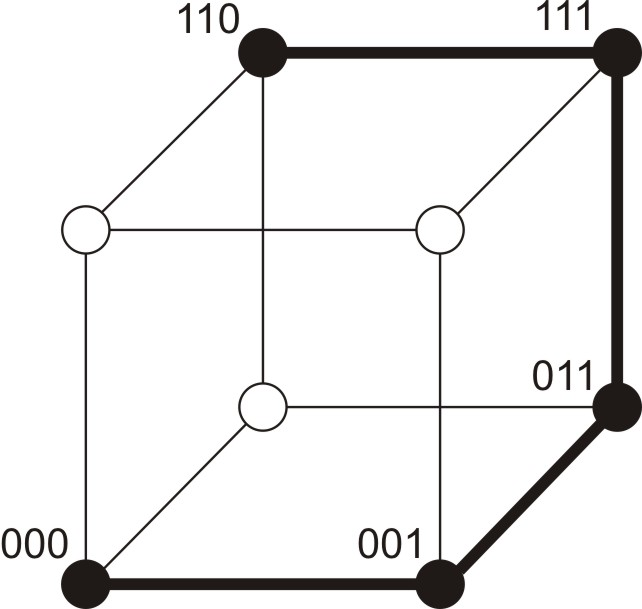
\includegraphics[scale=0.6]{img/Q3_long_path.jpg}
     \hspace*{12pt}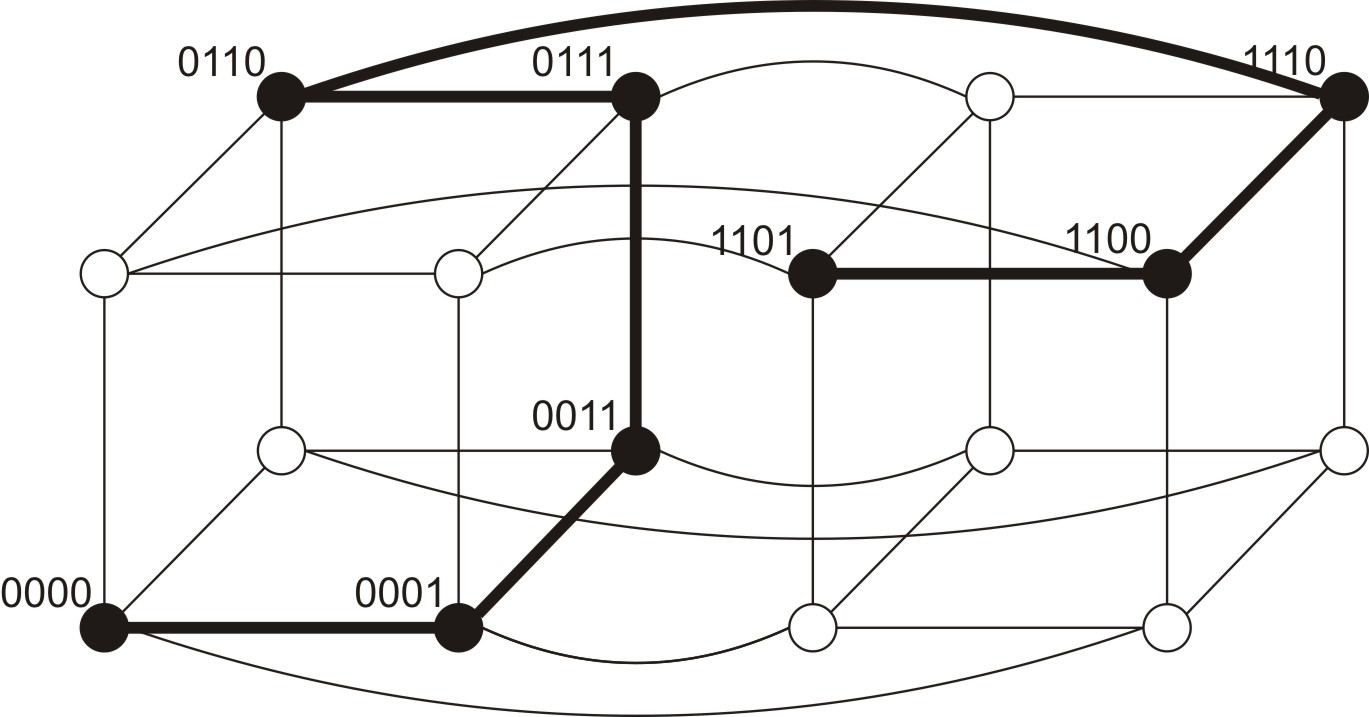
\includegraphics[scale=0.6]{img/Q4_long_path.jpg}\newline
     Dla tak małych wymiarów jest to jedyny z dokładnością do wyboru punktu początkowego i przepermutowania współrzędnych sposób uzyskania ścieżki tej długości.
     Już na tych przypadkach widać, że ścieżka tak powstała wygląda identycznie od początku i od końca
     (przy zamianie punktów początkowego i końcowego oraz przepermutowaniu współrzędnych). Dodatkowo widać też,
     że tylko 3 podkostki $Q_{n-2}$ zawierają wybrane do ścieżki wierzchołki, dokładniej pierwsza podkostka zawiera $P_{n-2}$, druga $P_{n-3}$
     i trzecia znów $P_{n-2}$ (znów "z dokładnością").\newline
     Konstrukcja indukcyjna $P_n$ przebiega następująco:\newline
     Startuję od $P_{n-1}$, który nie używa tylko współrzędne od $0$ do $n-2$, kolejnym wierzchołkiem w ciągu będzie sąsiad aktualnie ostatniego w kierunku
     $n-1$. Mam dane już ponad pół kostki, jeśli więc chcę uzyskać $P_n$ takie samo od początku jak i od końca wystarczy znaleźć odpowiednnią permutację.
     Co do tej nowej części mamy pewną dowolność przy wyborze permutacji, jednak musi się ona zgadzać na tej środkowej części
     ($P_{n-2}$ zaczynające się po krawędzi w kierunku $n-3$, a kończące przed dostawioną $n-2$ -- te współrzędne zostaną ze sobą zamienione w permutacji
     i w całej ścieżce $P_n$ krawędzie w tych kierunkach występują tylko po razie). Z kroku indukcyjnego $P_{n-2}$ jest symetryczne w ten sposób,
     więc istnieje odpowiednia permutacja na kierunkach w niej używanych, wystarczcy więc ją rozszerzyć od tą zamianę $n-1$ z $n-2$
     (i formalnie dowolnie uzupełnić o kierunki w niej nie występujące, choć tak na prawdę takich nie ma).
     Z konstrukcji wynika, że zbudowana tak ścieżka posiada własność: dowolne dwa wierzchołki ze ścieżki są sąsiadami w hiperkostce
     tylko wtedy gdy są sąsiadami na ścieżce wewnątrz trzech swoich części. Pomiędzy pierwszą i drugą częścią własność ta jest spełniona z kroku indukcyjnego,
     zaś pomiędzy trzecią i drugą jest tak samo z symetrii. Pozostają części pierwsza i trzecia, ale skoro są one całkowicie zanurzone w dwóch podkostkach,
     które nie mają między sobą krawędzi, to warunek ten jest również spełniony w tym przypadku.
    \end{proof}
    \begin{corollary}\label{fibo -> wykladniczy}
     Jako, że ciąg Fibonacciego rośnie w tempie wykładniczym -- ilość użytych wierzchołków wynosi
     $\frac{1}{\sqrt{5}}((\frac{1+\sqrt{5}}{2})^{n+1}-(\frac{1-\sqrt{5}}{2})^{n+1})\approx \frac{(1.62)^{n+1}}{\sqrt{5}}=\Omega(1.61^n)$, przy wielkości kostki $2^n$.
    \end{corollary}
   \section{Wyniki eksperymentalne}
    \begin{remark}\label{da sie dluzsze}
     Dla wymiarów większych niż $4$ da się otrzymać ścieżki jeszcze dłuższe -- dla $n=5$ najdłuższa możliwą ścieżką jest:\newline
     00000
     00001
     00011
     00111
     01111
     01110
     01100
     11100
     11101
     11001
     11011
     11010
     10010
     10110.\newline
     Ma ona długość 13, jest więc o 1 dłuższa od ścieżki otrzymanej na podstawie twierdzenia \ref{co najmniej fibo}
    \end{remark}
    Aby znaleźć możliwie najdłuższe ścieżki dla większych $n$ przeprowadziłem eksperymenty przy pomocy komputera.
    Wyszukiwanie ścieżek prowadziłem startując od wierzchołka $(0,...,0)$ i dobierając do istniejącej ścieżki nowy wierzchołek,
    który jest sąsiadem aktualnego końca i nie jest sąsiadem żadnego poprzedniego, aż do momentu, gdy taki wybór nie jest możliwy 
    -- w ten sposób otrzymuje "grę". Znalezienie wszystkich możliwych ścieżek otrzymywalnych w ten sposób
    (a są to wszystkie takie poprawne ścieżki, które zaczynają się w wierzchołku $(0,...,0)$) otrzymywane jest poprzez przejrzenie
    drzewa gry, której wierzchołkami są ścieżki, zaś ścieżki w przodkach tego wierzchołka są jej prefiksami.
    Drzewo tej gry ma maksymalny stopień rozgałęzienia równy $n$, zaś głębokość $|P|$.\newline
    Daje to złożoność algotyrmu przeglądającego wszystkie ściężki mocno pesymistycznie ograniczoną przez $O(n^{|P|})$. Nawet po zastosowaniu
    różnych usprawnień, algorytm dokładny szybko staje się zbyt wolny, dlatego dla $n\ge7$ musiałem skorzystać z metod losowych.
    \subsection{NMCS}
     Aby otrzymać pewną ścieżke, która posiada tę właśność, że nie da się jej już wydłużyć do innej poprawnej można przeprowadzić zejście po drzewie
     od korzenia do liścia poprzez losowe wybieranie jednego z dzieci za każdym razem, gdy taki wybór jest możliwy.\newline
     Przeprowadzając odpowiedno dużo takich losowych zejść po drzewie i wybierając najdłuższą ścieżkę ze znalezionych możemy uzyskać już w miarę dobry
     wynik, istnieją jednak metody, które pozwalają na lepsze ukierunkowanie losowości.\newline
     Jedną z takich metod jest przeszukiwanie Monte Carlo polegające na tym, że mając dany stan gry (aktualną ścieżkę) dla każdego możliwego ruchu
     (wyboru kolejnego wierzchołka) szacujemy jego wartość poprzez uruchomienie przeszukiwania losowego w tym kierunku i następnie wybranie najlepszego z nich.
     Metoda ta jest wykorzystywana głównie w przeypadkach gier w tym takich, w których gracz ma tylko częściowy wpływ na rozgrywkę (istnieje przeciwnik),
     jednak w przypadku szukania możliwie długiej ścieżki również się sprawdza.
     
     Rozszerzenie tej metody zostało zaprezentowane w pracy \cite{NMCS} zwane Nested Monte Carlo Search, polegające na tym, że do oszacowania
     wartości możliwych ruchów zamiast zwykłych przeszukiwań losowych używamy zwykłego przeszukiwania Monte Carlo.
     Dokładniej metoda ta zakłada, że tworząc rozwiązanie przy pomocy NMCS z poziomem $k$ używamy do wyboru ruchu NMCS z poziomem $k-1$ i tak dalej rekurencyjnie
     aż do poziomu $0$, który oznacza przeszukiwanie losowe. Można to przedstawić następującym pseudokodem:\newline\newline%TODO znów zadbać, żey strona się nie łamała brzydko
     \hspace*{0pt}$NMCS(v,level)\{$\newline
     \hspace*{16pt}	while$(TRUE)\{$\newline
     \hspace*{32pt}		$val.push\_back(v);$\newline
     \hspace*{32pt}		if$(|v.children|==0)$ return $val;$\newline
     \hspace*{32pt}		if$(level==0)\{$\newline
     \hspace*{48pt}			$v=random(v.children);$\newline
     \hspace*{32pt}		$\}$else$\{$\newline
     \hspace*{48pt}			$best=-1;$\newline    
     \hspace*{48pt}			foreach$(u\in v.children)\{$\newline
     \hspace*{64pt}				$val2=NMCS(u,level-1);$\newline
     \hspace*{64pt}				if$(value(val2)>best)\{$\newline
     \hspace*{80pt}					$best=value(val2);$\newline
     \hspace*{80pt}					$move=u;$\newline
     \hspace*{64pt}				$\}$\newline
     \hspace*{48pt}			$\}$\newline
     \hspace*{48pt}			$v=u;$\newline
     \hspace*{32pt}		$\}$\newline
     \hspace*{16pt}	$\}$\newline
     \hspace*{0pt}$\}$
    \subsection{Uwagi praktyczne}
     Ze względu na ogromną różnicę w złożoności algorytmu $NMCS$ w zależności od użytego poziomu można wprowadzić lekką modyfikację -- w przypadku,
     gdy wyższy poziom jest zbyt kosztowny, zaś niższy za słaby zamiast uruchamiać program z niższym poziomem wiele razy można poszerzyć przeszukiwanie.
     Poszerzenie takie można łatwo uzyskać uruchamiając dla każdego dziecka symulację poziomu niżej nie raz a $T$ razy
     (plus uruchomienie algorytmu najwyższego pozmiou tyle razy).
     
     Mając na uwadze algorytm z tą modyfikacją można oszacować pesymistyczną złożoność algorytmu dla szukania długiej izolowanej ścieżki w hiperkostce
     w zależności od wymiaru $n$,poziomu $L$, liczby razy przy sprawdzaniu dzieci $T$ oraz oczekiwanej długości maksymalnej ścieżki $|P|$.
     Złożoność ta jest wyrażona poprzez równanie rekurencyjne:\newline
     $NMCS(n,0,T,|P|)=n\cdot T\cdot |P|$\newline
     $NMCS(n,L,T,|P|)=n\cdot T\cdot NMCS(n,L-1,T,|P|-1)+NMCS(n,L,T,|P|-1)$\newline
     Które daje rozwiązanie:\newline
     $NMCS(n,L,T,|P|)=O(T^{L+1}\cdot n^{L+1}\cdot|P|^{L+1})$     
     
     W przypadku szukania izolowanej ściezki w hiperkostce nalezy jeszcze doliczyć czas i pamięć potrzebne na sprawdzanie czy nowo wybrany (wylosowany)
     wierzchołek nie jest sąsiadem jednego z wierzchołków z początku ścieżki.
     
     Jedną z możliwych metod jest za każdym razem przeiterowanie po aktualnej ściężce i porównanie ciągów binarnych, daje to jednak złożoność
     czasową rzędu $n |P|$. Drugą metodą jest zapamiętywanie wszystkich sąsiadów wierzchołków ze ścieżki (plus ich samych) w tablicy binarnej rozmiaru $2^n$.
     W tym wypadku sprawdzanie jest trywialnie proste (w czasie potrzebnym na odczytanie nazwy wierzchołka),
     jednak złożoność pamięicowa w przypadku NMCS poziomu $0$ przeważa nad złożonością czasową samego algorytmu.
     W przypadku małych $n$ nie jest to jednak złe rozwiązanie, ponieważ ze względu na liczne optymalizacje tablic binarnych jest to najszybsze rozwiązanie.
     Trzecią (pośrednią) metodą jest użycie jako struktury drzewa prefiksowego lub tablicy hashującej uzyskując podobnie do tablicy binarnej
     złożoność $O(n)$ na odczytanie i wstawienie wierzchołka jednocześnie potrzebując jedynie $O(n^{1.5}\cdot|P|)$ lub $O(n\cdot|P|)$ pamięci w zależności od użytej struktury.
     
     W przypadku użycia struktury zapamiętującej sąsiadów wierzchołków ze ścieżki należy jeszcze zwrócić uwagę na zmienianie jej stanu przy wchodzeniu
     i wracaniu z niższych poziomów wywołania. Można albo za każdym razem pamiętać wszystkie wstawione wierzchołki i przy zwracaniu wyniku
     do poziomu wyżej dokonywać ich usunięcia, albo można za każdym razem kopiować całą strukturę (dosyć efektywne przy użyciu tablic).
     W drugim przypadku wystarczy mieć $L+1$ kopii stuktury na raz (po jednej na każdy poziom) i przy powrocie z apoziomu niżej
     zastępować starą wersję z tamtego poziomu kopią z poziomu o 1 wyżej.
     
     Mając to na uwadze można zaprogramować algorytm tak, aby miał złożoności czasową $O(T^{L+1}\cdot n^{L+2}\cdot|P|^{L+1})$
     i pamięciową $O(L\cdot n\cdot |P|)$.\newline
     
     Przeszukiwanie można dodatkowo zawęzić jeśli program weźmie pod uwagę, że kierunki, które nie pojawiły się jeszcze na ścieżce są równoważne
     (wystarczy pamiętać liczbę oznaczającą ilość kierunków już użytych i nie używać kierunków większych niż ta liczba + 1).
     W ten sposób ustalone są pierwsze 3 ruchy ($1\rightarrow2\rightarrow4\rightarrow8$ przy numerowaniu klasycznym),
     zaś na czwarty są tylko dwie możliwości ($8\rightarrow7,8\rightarrow17$). Daje to duże przyśpieszenie przy małych przypadkach,
     jednak przy większych nie ma już większego znaczenia.
    \subsection{Uzyskane wartości}
     Przy pomocy komputera i przedstawonych wyżej algorytmów przeprowadziłem przeszukiwanie w celu znalezienia możliwie najdłuższej takiej ścieżki.
     W przypadku $n\le6$ przy pomocy pełnego przeszukiwania, a dalej NMCS z 4 poziomami dla $n=7$, 3 dla $n=8$, 2 dla $9\le n\le12$ i 1 dla $13\le n\le18$
     z ilością wywołań niższego poziomu takich żeby podobny był czas dla wszystkich $n$. Dalej użyłem zwykłego błądzenia losowego i wybierania najdłuższej
     uzyskanej tak ścieżki (ilość przeszukiwań znów dostosowana do tego czasu).
     Program użyty do takiego przeszukiwania wraz z zapisami ścieżek dla mniejszych $n$ (dla większych brak ze względu na wielkość plików)
     i dokładnymi parametrami jest dołączony do pracy.\newline
     
     Poniższa tabelka i wykres logarytmiczny prezentują porównanie najlepszych rezultatów uzyskanych dla poszczególnych $n$ ($|P|$) do wielkości ścieżki
     Fibonacciego i całego grafu.
     $\begin{array}{|c|c|c|c|c|c|c|c|c|c|c|c|c|c|c|}
      \hline
      n&0&1&2&3&4&5&6&7&8&9&10&11&12&13\\
      \hline
      F_{n+1}&1&2&3&5&8&13&21&34&55&89&144&233&377&610\\
      \hline
      |P|+1&1&2&3&5&8&14&27&51&86&146&245&423&749&1373\\
      \hline
      2^n&1&2&4&8&16&32&64&128&256&512&1024&2048&4096&8192\\
      \hline
      \sqrt[n]{|P|+1}&&2&1.73&1.71&1.68&1.7&1.73&1.75&1.75&1.74&1.73&1.73&1.74&1.74\\
      \hline
     \end{array}$\newline
     $\begin{array}{|c|c|c|c|c|c|c|c|c|c|}
      \hline
      n&14&15&16&17&18&19&20&21&22\\
      \hline
      F_{n+1}&987&1597&2584&4181&6765&10946&17711&28657&46368\\
      \hline
      |P|+1&2568&4778&9017&16612&28287&34801&63271&118344&216033\\
      \hline
      2^n&16384&32768&65536&131072&262144&524288&1048576&2097152&4194304\\
      \hline
      \sqrt[n]{|P|+1}&1.75&1.76&1.77&1.77&1.77&1.73&1.74&1.74&1.75\\
      \hline
     \end{array}$\newline
     $\begin{array}{|c|c|c|c|c|c|c|c|}
      \hline
      n&23&24&25&26&27&28&29\\
      \hline
      F_{n+1}&75025&121393&196418&317811&514229&832040&1346269\\
      \hline
      |P|+1&410719&748502&1373384&2543441&4774783&9098482&16788856\\
      \hline
      2^n&8388608&16777216&33554432&67108864&134217728&268435456&536870912\\
      \hline
      \sqrt[n]{|P|+1}&1.75&1.76&1.76&1.76&1.77&1.77&1.77\\
      \hline
     \end{array}$\newline
      $\begin{array}{|c|c|c|c|c|c|}
      \hline
      n&30&31&32&33&34\\
      \hline
      F_{n+1}&2178309&3524578&5702887&9227465&14930352\\
      \hline
      |P|+1&32747927&61637291&117676035&204031449&386051791\\
      \hline
      2^n&1073741824&2147483648&4294967296&8589934592&17179869184\\
      \hline
      \sqrt[n]{|P|+1}&1.78&1.78&1.79&1.79&1.79\\
      \hline
     \end{array}$\newline
     \begin{center}
      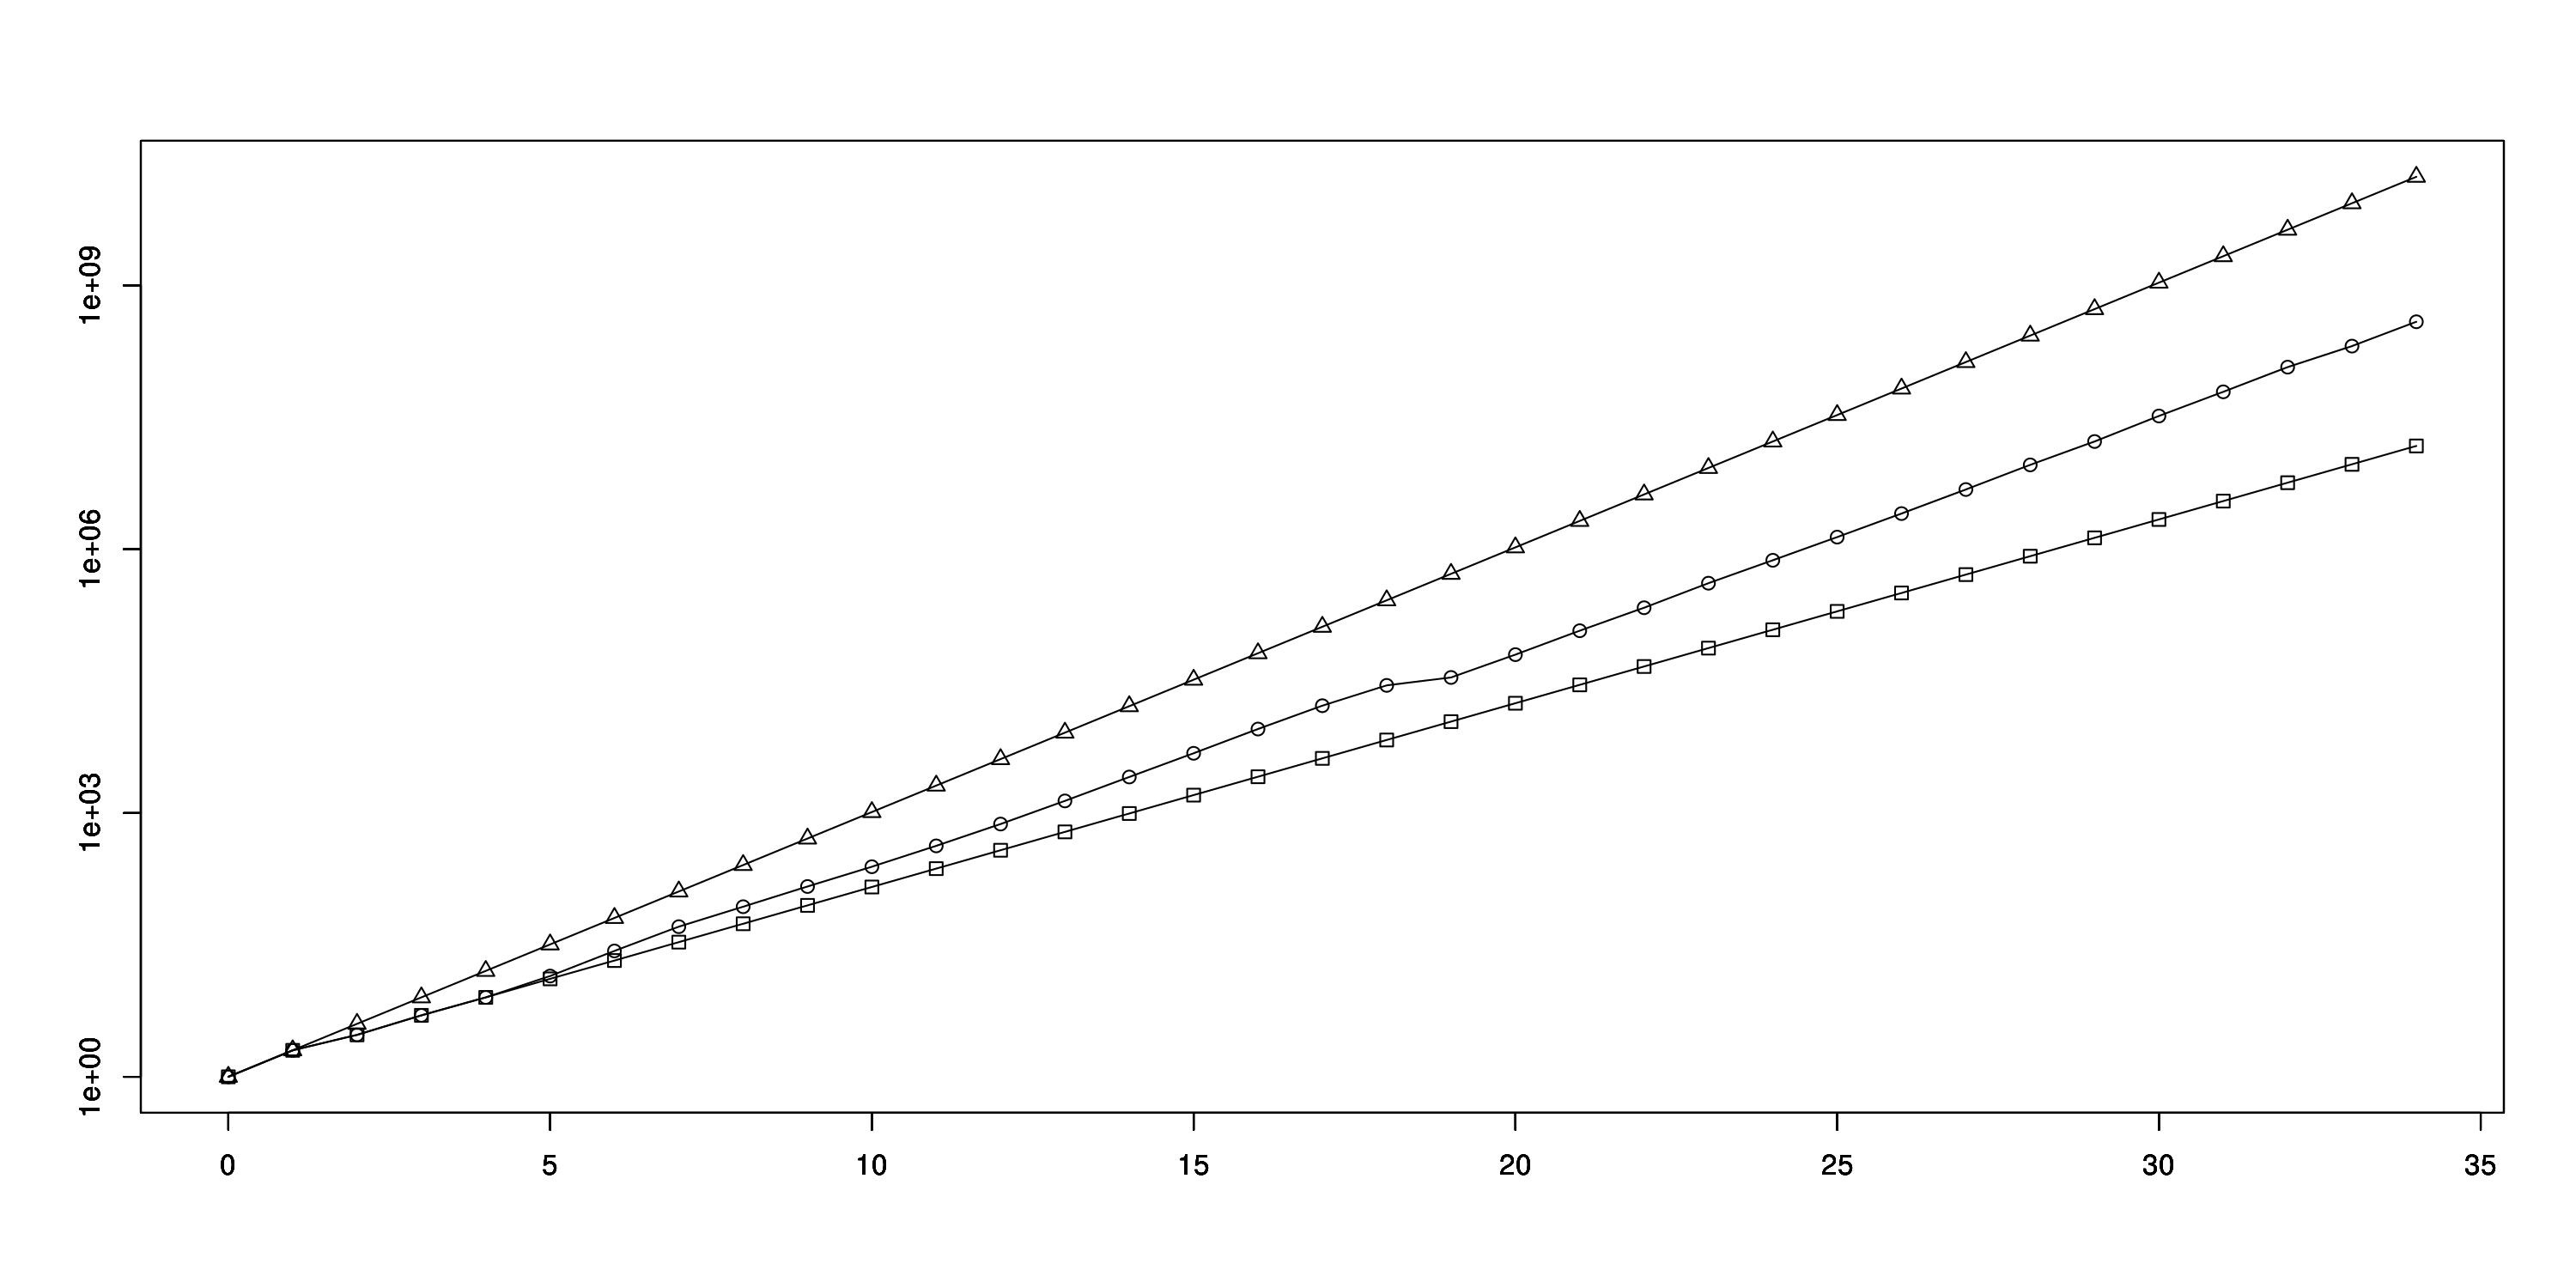
\includegraphics[scale=0.37]{img/plot1.jpg}
     \end{center}

    
 
    %TODO sprobowac sprawdzic czy nie da sie opisac zbioru nieodwiedzanych przez dluga sciezke - ktory jest wielomianowy (rozdzial o dlugich sciezkach i cyklach)
  
  
\begin{thebibliography}{99}%TODO dziwne litery , upcase?
\addcontentsline{toc}{chapter}{Bibliografia}

  \bibitem{LPV} L. Lovasz, J. Pelikan and K. Vesztergombi.
   "Discrete Mathematics, Elementary and Beyond."
   \textit{Undergraduate Texts in Mathematics. New York: Springer, first edition, 2003}   

  \bibitem{HAR} L. H. HARPER,
   "Optimal Numberings and Isoperimetric Problems on Graphs"
   \textit{JOURNAL OF COMBINATORIAL THEORY 1, 385-393 (1966)}
   
  \bibitem{DFGKR} Tomas Dvorak, Jirı Fink, Petr Gregor, Vaclav Koubek and Tomasz Radzik,
   "Efficient connectivity testing of hypercubic networks with faults"
   
  \bibitem{FG} Jirı Fink and Petr Gregor,
   "Long paths and cycles in hypercubes with faulty vertices"
   
  \bibitem{Wie} G. Wiener,
   "Edge multiplicity and other trace functions."
   \textit{In Proceedings of European Conferenc on Combinatorics, Graph Theory and Applications (EuroComb 2007), volume 29 of
   Electronic Notes in Discrete Mathematics, pages 491–495, 2007.}
   
  \bibitem{FG2} Jirı Fink and Petr Gregor,
   "Long pairs of paths in faulty hypercubes"
  
  \bibitem{Locke} Nelson Casenada and Ivan S. Gotchev,
   "Proof of Locke's Conjecture, I"

  \bibitem{Pegr} David Pegrimek,
   "Hamiltonian cycles in hypercubes with removed vertices",
   \textit{Prague 2013}
  
  \bibitem{SCJY}Sun, Chao-Ming and Jou, Yue-Dar,
   "Hamiltonian laceability of hypercubes with some faulty elements",
   \textit{In Proceedings of 2009 IEEE International Conference on Networking, Sensing and Control, Okayama, Japan,
   March 26-29, 2009, pp.626-630}
  
   %------------------------------------------------------------pompowanie
   
  \bibitem{NMCS} Tristan Cazenave,
   "Nested Monte-Carlo Search"
   \textit{LAMSADE Universite Paris-Dauphine Paris, France}   
   
  \bibitem{HHH} Frank Harary, John P. Hayes and Horng--Jyh Wu,
   "A survey of theory of hypercube graphs"
   \textit{Comput. Math. Applic. Vol. 15, No 4, pp. 277-289, 1988}
   
  \bibitem{HL} Frank Harary, Marilynn Livingston,
   "Independent domination in hypercubes"
   \textit{Appl. Math. Lett. Vol. 6, No 3, pp. 27-28, 1993}
   
  \bibitem{RS} Wojciech Rytter $\&$ Bartosz Szreder,
   "Wprowadzenie do kombinatoryki algorytmicznej"
   
  \bibitem{Knuth} DONALD E. KNUTH,
   "Generating All Tuples and Permutations"
   \textit{THE ART OF COMPUTER PROGRAMMING VOLUME 4, FASCICLE 2}
  
  \bibitem{Ruskey} FRANK RUSKEY,
   "Combinatorial Generation"
   \textit{Working Version, October 1, 2003}

  \bibitem{SW} Tibor Szabo, Emo Weltz,
   "Unique Sink Orientations of Cubes"
   
  \bibitem{Wong} Chi Him Wong,
   "Novel universal cycle constructions for a variety of combinatorial objects"
   \textit{Guelph, Ontario, Canada, April, 2015}
   
\end{thebibliography}

\end{document}